% This is CystoDS_LNCS_Paper_VI.tex
% Scientific Manuscript formatted in Springer LNCS style
% 100% Compatible with Overleaf (pdfLaTeX, XeLaTeX, LuaLaTeX) and Tectonic
% Body discussion: High-density, rigorous academic Vietnamese (Q1 Journal Standard)
% All Tables, Figures, Captions, Headers, and Technical Notations: 100% English
%
\documentclass[runningheads]{llncs}
%
\usepackage{iftex}
\ifPDFTeX
  \usepackage[utf8]{inputenc}
  \usepackage[T1,T5]{fontenc}
  \usepackage[english,vietnamese]{babel}
  \DeclareUnicodeCharacter{00D7}{\ensuremath{\times}}
  \DeclareUnicodeCharacter{00B1}{\ensuremath{\pm}}
  \DeclareUnicodeCharacter{2264}{\ensuremath{\le}}
  \DeclareUnicodeCharacter{2265}{\ensuremath{\ge}}
  \DeclareUnicodeCharacter{2192}{\ensuremath{\to}}
  \DeclareUnicodeCharacter{2026}{\dots}
\else
  \usepackage{fontspec}
\fi

\usepackage{amsmath,amssymb}
\usepackage{graphicx}
\graphicspath{{./}{paper_assets/}{./paper_assets/}}
\usepackage{booktabs}
\usepackage{array}
\usepackage{tabularx}
\usepackage{adjustbox}
\usepackage{multirow}
\usepackage{makecell}
\usepackage{url}
\usepackage{cite}
\usepackage{float}
\usepackage{placeins}
\usepackage{hyperref}
\hypersetup{
    colorlinks=true,
    linkcolor=blue,
    filecolor=magenta,      
    urlcolor=cyan,
    citecolor=blue,
}

% Typography customizations: English Tables and Figures, Vietnamese Abstract
\providecommand{\abstractname}{Tóm tắt}
\providecommand{\keywordname}{{\bfseries Từ khóa:}}
\renewcommand{\figurename}{Fig.}
\renewcommand{\tablename}{Table}
\providecommand{\refname}{Tài liệu tham khảo}

\begin{document}
%
\title{CystoHier: Khung học phân cấp tách rời cho bài toán phân loại tổn thương nội soi bàng quang trên dữ liệu mất cân bằng dài đuôi}
%
\titlerunning{CystoHier: Phân loại phân cấp nội soi bàng quang dài đuôi}
%
\author{Nguyễn Xuân Cường\inst{1}\orcidID{0000-0002-1825-0097} \and
Võ Quốc Trình\inst{1}\orcidID{0000-0002-8877-6655}}
%
\authorrunning{N. X. Cường và V. Q. Trình}
%
\institute{Trường Đại học FPT, Phân hiệu Đà Nẵng, Đà Nẵng, Việt Nam\\
\email{cuongnxde180528@fpt.edu.vn}}
%
\maketitle              % typeset the header of the contribution
%
\begin{abstract}
Nội soi bàng quang (Cystoscopy) là tiêu chuẩn vàng trong tầm soát, chẩn đoán và theo dõi ung thư biểu mô đường niệu (Bladder Cancer). Tuy nhiên, việc xây dựng các hệ thống trí tuệ nhân tạo (AI) hỗ trợ phẫu thuật viên đối mặt với hai thách thức cốt lõi: cấu trúc phân cấp chẩn đoán y học đa tầng (nhị phân, nhóm bệnh cảnh thô và phân loại chi tiết) và hiện tượng mất cân bằng phân phối dài đuôi cực đoan (Extreme Long-Tailed Imbalance) khi các tổn thương ác tính hoặc bệnh lý hiếm chỉ xuất hiện ở một số ít bệnh nhân. Bài báo này đề xuất \textbf{CystoHier} -- một khung học phân cấp tách rời ba giai đoạn toàn diện trên nền tảng kiến trúc Swin Transformer nhằm giải quyết sự đánh đổi giữa học biểu diễn đặc trưng và tối ưu hóa ranh giới phân loại đa tầng. Các đóng góp cốt lõi của \textbf{CystoHier} bao gồm: (1) Kiến trúc đa nhiệm chia sẻ biểu diễn sâu (\textit{Shared Late-Stage Multi-Head Backbone}); (2) Hàm mất mát \textit{Smoothed Balanced Softmax} (SBS) với tiên nghiệm mượt theo số lượng bệnh nhân thực tế nhằm giảm thiểu thiên lệch lấy mẫu; (3) Tinh chỉnh co cụm không gian đặc trưng bằng \textit{Supervised Contrastive Loss} ($\mathcal{L}_{\text{supcon}}$); (4) Ràng buộc nhất quán phả hệ với lịch trình \textit{Curriculum Hierarchy Warmup} giúp giải phóng thắt cổ chai biểu diễn ở giai đoạn sớm; (5) Chiến lược huấn luyện tuần tự ba giai đoạn tách rời (\textit{Three-Stage Decoupled Training}) với cơ chế đóng băng tham số (\textit{Parameter-Isolated Representation Preservation}); (6) Cơ chế suy luận kết hợp \textit{Hierarchical Marginalization \& Multi-Head Blending} tích lũy xác suất từ 22 phân lớp chi tiết về 5 nhóm thô; và (7) Đánh giá ngoại kiểm độc lập (\textit{External Cohort Validation}) trên bộ dữ liệu Lazo et al. (1.754 ảnh, 23 bệnh nhân). Đánh giá thực nghiệm trên bộ dữ liệu CystoDS (8.067 ảnh, 160 bệnh nhân) theo giao thức 3-Fold Patient-Disjoint Hold-out (100\% độc lập bệnh nhân) cho thấy \textbf{CystoHier} đạt hiệu năng cao nhất trong số các mô hình đối chuẩn: Binary AUROC \textbf{0,9986 $\pm$ 0,0002}, Coarse Accuracy \textbf{86,42\% $\pm$ 3,52\%}, Fine Macro-F1 (Supported) \textbf{0,6450 $\pm$ 0,1105}, và tính nhất quán Coarse-Fine đạt \textbf{89,52\% $\pm$ 3,80\%} trên tập kiểm định độc lập. Đánh giá zero-shot trên tập ngoại kiểm Lazo et al. xác nhận khả năng tổng quát hóa vững chắc (AUROC 0,9587 $\pm$ 0,0118, Accuracy 85,37\% $\pm$ 2,05\%), đặc biệt cải thiện độ nhạy phát hiện tổn thương không tạo u NTL (46,02\% vs 39,05\%) và ảnh NBI (Accuracy 81,00\% vs 76,01\%). Bản đồ nhiệt Grad-CAM cải thiện độ trùng khớp IoU giải phẫu từ 5,00\% lên 23,56\% trên mặt nạ chuyên gia, đồng thời đạt thông lượng suy luận thời gian thực 66,7 FPS end-to-end trên phần cứng biên, chứng minh tính khả thi của phương pháp học phân cấp dài đuôi cho chẩn đoán nội soi bàng quang.

\keywords{Cystoscopy \and Bladder Cancer \and Hierarchical Classification \and Long-Tailed Learning \and Vision Transformer \and Contrastive Learning \and Curriculum Warmup \and External Validation \and Grad-CAM.}
\end{abstract}
%
%
%
\section{Mở đầu}
\label{sec:intro}

Ung thư bàng quang (Bladder Cancer) là một trong mười bệnh lý ác tính phổ biến nhất trên toàn cầu, với hơn 570.000 ca mắc mới và 212.000 ca tử vong mỗi năm \cite{ref_lee2026cystods,ref_shkolyar2019augmented}. Nội soi bàng quang ánh sáng trắng (White Light Cystoscopy -- WLC) kết hợp nội soi dải tần hẹp (Narrow Band Imaging -- NBI) là phương pháp tiêu chuẩn vàng giúp phẫu thuật viên phát hiện sớm tổn thương niêm mạc, định hướng sinh thiết và thực hiện phẫu thuật cắt đốt u nội soi qua niệu đạo (Transurethral Resection of Bladder Tumor -- TURBT) \cite{ref_wu2022multicenter,ref_wang2026narrowband}. Tuy nhiên, quy trình chẩn đoán qua nội soi phụ thuộc lớn vào kinh nghiệm và sự tập trung của bác sĩ, dễ dẫn đến tỷ lệ bỏ sót các tổn thương phẳng như ung thư biểu mô tại chỗ (Carcinoma in Situ -- CIS) lên tới 10--20\%, đồng thời tạo ra tỷ lệ dương tính giả cao do niêm mạc viêm mạn tính hoặc các mốc giải phẫu tự nhiên \cite{ref_shkolyar2019augmented,ref_zhang2026multiarch}.

Trong thực hành lâm sàng, quy trình chẩn đoán nội soi bàng quang mang tính \textbf{phân cấp tự nhiên (Diagnostic Hierarchy)} gồm 3 mức độ:
\begin{enumerate}
    \item \textbf{Tầng 1 -- Nhị phân (Binary Detection):} Xác định nhanh vùng nghi ngờ tổn thương (Region of Interest -- ROI) so với vùng bình thường hoặc dị vật (Non-ROI) để cảnh báo tức thời cho phẫu thuật viên.
    \item \textbf{Tầng 2 -- Phân nhóm bệnh lý thô (Coarse Grouping):} Phân loại thành 5 nhóm bệnh cảnh lâm sàng lớn: Ác tính (\textit{Malignant}), Không ác tính (\textit{Non-malignant}), Niêm mạc bình thường (\textit{Normal mucosa}), Mốc giải phẫu (\textit{Anatomical landmarks}), và Dị vật/Dụng cụ can thiệp (\textit{Foreign bodies/Artefacts}).
    \item \textbf{Tầng 3 -- Định danh phân lớp chẩn đoán chi tiết (Fine-Grained Diagnostic Classification):} Nhận diện chính xác 22 phân lớp chi tiết (gồm các dạng tổn thương ác tính như \textit{HighGradePapillary}, \textit{LowGradePapillary}, \textit{CIS}; dạng viêm/lành tính; các mốc giải phẫu và dị vật can thiệp) nhằm phục vụ quyết định can thiệp phẫu thuật chính xác.
\end{enumerate}

Mặc dù việc phân loại đa tầng mang lại giá trị lâm sàng vượt bậc, việc huấn luyện mô hình học sâu đối mặt với hiện tượng \textbf{mất cân bằng phân phối dài đuôi cực đoan (Extreme Long-Tailed Distribution)} \cite{ref_lee2026cystods}. Cụ thể, trong bộ dữ liệu CystoDS \cite{ref_lee2026cystods}, lớp niêm mạc bình thường chiếm áp đảo tới 79,16\% (6.386/8.067 ảnh), trong khi nhiều phân lớp ác tính và tổn thương hiếm (như CIS, PreMalignant, BenignRare) chỉ xuất hiện ở từ 1 đến 6 bệnh nhân.

Khi giải quyết bài toán này, các phương pháp hiện hành bộc lộ ba mâu thuẫn kỹ thuật cốt lõi:
\begin{itemize}
    \item \textbf{Mâu thuẫn 1 -- Xung đột giữa học biểu diễn và cân bằng phân loại (Representation vs. Classifier Trade-off):} Huấn luyện đa nhiệm một giai đoạn đồng thời (1-Stage Joint) với các hàm mất mát đuôi dài mạnh (như Balanced Softmax \cite{ref_ren2020balanced}) tạo ra gradient lớn từ các lớp đuôi, làm méo mó không gian đặc trưng tổng quát và làm suy giảm độ chính xác của các lớp đa số và lớp thô \cite{ref_kang2020decoupling}.
    \item \textbf{Mâu thuẫn 2 -- Thắt cổ chai phân cấp sớm (Early Hierarchy Bottleneck):} Việc áp đặt ràng buộc phả hệ cứng ($L_{\text{hierarchy}}$) ngay từ những epoch đầu tiên gò bó không gian biểu diễn của mạng xương sống (Backbone), cản trở việc học các đặc trưng thị giác biểu mô cơ bản \cite{ref_liu2021swin}.
    \item \textbf{Mâu thuẫn 3 -- Nguy cơ trôi dạt ranh giới quyết định (Decision Boundary Drift) khi tinh chỉnh phân tách:} Khi tinh chỉnh đầu phân loại chi tiết (Fine Head) ở giai đoạn sau, nếu không có cơ chế cố định biểu diễn và cô lập tham số các đầu phân loại tầng trên, ranh giới quyết định của tầng Binary và Coarse sẽ bị ảnh hưởng tiêu cực.
\end{itemize}

Nhằm giải quyết các hạn chế trên, nghiên cứu này đề xuất khung phương pháp \textbf{CystoHier} trên nền tảng kiến trúc Swin Transformer \cite{ref_liu2021swin}. Bài báo đóng góp các giá trị khoa học cốt lõi sau:
\begin{enumerate}
    \item \textbf{Kiến trúc đa nhiệm Shared Late-Stage Multi-Head:} Thiết kế trích xuất đặc trưng chung ở Stage 4 sâu nhất (vector $z \in \mathbb{R}^{768}$) cung cấp trường tiếp nhận toàn cảnh và độ bền vững trước nhiễu lóa sáng nội soi.
    \item \textbf{Hàm mất mát Smoothed Balanced Softmax theo tiên nghiệm bệnh nhân:} Đề xuất công thức điều hòa logit dựa trên căn bậc hai số lượng bệnh nhân thực tế ($\pi_j = \text{patients}_j^{0{,}5}$), giảm thiểu sai số do phân bố ảnh lặp lại ở cấp bệnh nhân.
    \item \textbf{Không gian biểu diễn tăng cường Supervised Contrastive Regularization:} Tích hợp $\mathcal{L}_{\text{supcon}}$ giúp co cụm các tổn thương cùng phân lớp chi tiết và tách biệt ranh giới biểu mô trong không gian ẩn.
    \item \textbf{Lịch trình Curriculum Hierarchy Warmup:} Cơ chế tăng dần trọng số ràng buộc phả hệ từ $0 \to 0{,}25$ trong 12 epochs đầu, giải phóng không gian đặc trưng ở giai đoạn khởi tạo.
    \item \textbf{Chiến lược tinh chỉnh tách rời ba giai đoạn (3-Phased Sequential Training):} Tách bạch: \textit{Representation Learning} $\to$ \textit{Coarse Alignment} $\to$ \textit{Fine Alignment} với cơ chế cô lập tham số bảo toàn biểu diễn (\textit{Parameter-Isolated Representation Preservation}).
    \item \textbf{Cơ chế suy luận Hierarchical Marginalization \& Blending:} Tích lũy xác suất từ 22 lớp con chi tiết về 5 nhóm cha kết hợp hòa trộn ($\lambda=0{,}25$), tăng Coarse Accuracy thêm $+5{,}24\%$ trên tập Test độc lập.
    \item \textbf{Khảo sát đối chuẩn toàn diện về Backbone và Loss:} Sàng lọc hệ thống 4 họ kiến trúc mạng thị giác và 7 hàm mất mát xử lý phân phối dài đuôi qua 3 phân hoạch hold-out 100\% độc lập bệnh nhân.
    \item \textbf{Đánh giá ngoại kiểm độc lập (External Validation):} Khảo sát trực tiếp mô hình trên toàn bộ 1.754 ảnh / 23 bệnh nhân của bộ dữ liệu Lazo et al. \cite{ref_lazo2023semisupervised} nhằm kiểm chứng năng lực tổng quát hóa zero-shot.
\end{enumerate}

\section{Các công trình liên quan}
\label{sec:related_work}

\subsection{Học sâu trong chẩn đoán hình ảnh nội soi bàng quang}
Trong những năm gần đây, nhiều nghiên cứu đã ứng dụng mạng nơ-ron tích chập (CNN) và Vision Transformer vào bài toán nội soi bàng quang. Shkolyar và cộng sự (2019) \cite{ref_shkolyar2019augmented} đã phát triển hệ thống CystoNet phát hiện khối u bàng quang trên video WLC với độ nhạy 90,9\% và độ đặc hiệu 98,6\%. Wu và cộng sự (2022) \cite{ref_wu2022multicenter} thực hiện nghiên cứu đa trung tâm quy mô lớn trên 69.204 ảnh nội soi nhằm phân loại nhị phân tổn thương ác tính và lành tính. Lazo và cộng sự (2023) \cite{ref_lazo2023semisupervised} đề xuất mô hình bán giám sát phân loại 4 nhóm mô trên 1.754 ảnh WLC/NBI. Jia và cộng sự (2023) \cite{ref_jia2023transformer} tích hợp Transformer nâng cao độ chính xác phát hiện u. Gần đây, Abd El-Aziz và cộng sự (2025) \cite{ref_abdelaziz2025efficientnet} sử dụng EfficientNet-B3 phân loại mô bàng quang, và Wang và cộng sự (2026) \cite{ref_wang2026narrowband} xây dựng hệ thống chẩn đoán đa trung tâm dựa trên ảnh nội soi NBI.

Nghiên cứu công bố bộ dữ liệu CystoDS của Lee và cộng sự (2026) \cite{ref_lee2026cystods} đã thiết lập chuẩn đánh giá trên 8.067 ảnh nội soi. Tuy nhiên, nghiên cứu gốc chỉ khảo sát bài toán phân loại nhị phân phẳng (ROI Detection) trên một phân hoạch đơn lẻ, hoàn toàn chưa khai thác cấu trúc phân cấp 5 nhóm Coarse và 22 phân lớp chẩn đoán chi tiết.

\subsection{Học phân loại phân cấp và phân phối mất cân bằng dài đuôi}
Học phân cấp (Hierarchical Classification) khai thác cấu trúc cây phả hệ y học để áp đặt tính nhất quán ngữ nghĩa, đảm bảo rằng một mẫu được dự đoán là lớp con chi tiết thì bắt buộc phải thuộc về nhóm cha tương ứng \cite{ref_lazo2023semisupervised}. 

Đối với bài toán mất cân bằng phân phối dài đuôi (Long-Tailed Learning), các kỹ thuật truyền thống bao gồm tái lấy mẫu (Re-sampling) và tái đánh trọng số (Cost-sensitive Re-weighting) \cite{ref_ren2020balanced}. Kang và cộng sự (2020) \cite{ref_kang2020decoupling} chứng minh rằng việc tách rời quy trình học đặc trưng và cân bằng bộ phân loại (Decoupled Training / cRT) mang lại hiệu quả vượt trội. Ren và cộng sự (2020) \cite{ref_ren2020balanced} đề xuất Balanced Softmax nhằm dịch chuyển biên phân loại theo xác suất tiên nghiệm của nhãn, trong khi Menon và cộng sự (2021) \cite{ref_menon2021logit} xây dựng cơ sở lý thuyết cho Logit Adjustment. Trong nghiên cứu này, chúng tôi phát triển khung phương pháp \textbf{CystoHier} kết hợp toàn diện các cơ chế trên nhằm giải quyết trọn vẹn cả ba thách thức: phân cấp, dài đuôi và bảo toàn biểu diễn.

\begin{table}[t]
\centering
\caption{Summary and comparison of related deep learning studies in bladder cystoscopy image analysis.}
\label{tab:related_work}
\begin{adjustbox}{max width=\textwidth}
\begin{tabular}{lccccc}
\toprule
\textbf{Study / Reference} & \textbf{Dataset / Sample Size} & \textbf{Taxonomy / Levels} & \textbf{Patient-Disjoint} & \textbf{Core Methodology} & \textbf{Primary Limitation} \\
\midrule
Lee et al. (CystoDS) \cite{ref_lee2026cystods} & 8,067 images / 160 Pts & 1 level (2 classes ROI) & Single Split & Swin-Large Baseline & Binary only, ignores 5 Coarse / 22 Fine \\
Shkolyar et al. \cite{ref_shkolyar2019augmented} & Internal WLC Video & 1 level (Tumor Detection) & Yes & CNN Object Detection & No fine-grained classification \\
Wu et al. \cite{ref_wu2022multicenter} & 69,204 images / 10,729 Pts & 1 level (Malignant vs Benign) & Multicenter & CNN Classifier & Flat binary, lacks fine diagnostic depth \\
Lazo et al. \cite{ref_lazo2023semisupervised} & 1,754 images / 23 Pts & 1 level (4 tissue classes) & Yes & Semi-supervised CNN & Small cohort, lacks hierarchical tree \\
Wang et al. \cite{ref_wang2026narrowband} & Multicenter NBI & 2 levels (Tumor / Grade) & Yes & Multitask CNN & Strictly requires NBI hardware \\
\textbf{Ours (CystoHier)} & \textbf{8,067 images / 160 Pts} & \textbf{3 levels (2 / 5 / 22 classes)} & \textbf{3-Split Standardized} & \textbf{CystoHier (3S + Ens.)} & \textbf{Simultaneously solves 3-level taxonomy \& tail} \\
\bottomrule
\end{tabular}
\end{adjustbox}
\end{table}

\section{Tập dữ liệu CystoDS và Giao thức Nghiên cứu}
\label{sec:dataset}

\subsection{Thống kê ba tầng phân cấp của bộ dữ liệu CystoDS}
Bộ dữ liệu CystoDS \cite{ref_lee2026cystods} bao gồm tổng cộng 8.067 ảnh nội soi WLC thu nhận từ 160 bệnh nhân duy nhất, được gắn nhãn đồng thời ở 3 cấp độ chẩn đoán y khoa (Table~\ref{tab:dataset_stats}):
\begin{itemize}
    \item \textbf{Tầng 1 (Binary -- 2 lớp):} 1.219 ảnh tổn thương (\textit{ROI}: Malignant + Non-malignant) và 6.848 ảnh không tổn thương (\textit{Non-ROI}: Normal mucosa + Landmarks + Foreign bodies).
    \item \textbf{Tầng 2 (Coarse -- 5 nhóm):} \textit{Malignant} (998 ảnh), \textit{Non-malignant} (221 ảnh), \textit{Normal mucosa} (6.386 ảnh), \textit{Anatomical landmarks} (211 ảnh), và \textit{Foreign bodies} (251 ảnh).
    \item \textbf{Tầng 3 (Fine -- 22 phân lớp chẩn đoán chi tiết):} Gồm 4 phân lớp ác tính (\textit{LowGradePapillary}, \textit{HighGradePapillary}, \textit{CIS}, \textit{PreMalignant}), 8 phân lớp lành tính/viêm (\textit{BenignNOS}, \textit{InflammationNOS}, \textit{CCG}, \textit{Denuded}, \textit{UrothelialPapilloma}, \textit{SquamousMetaplasia}, \textit{NephrogenicAdenoma}, \textit{BenignRare}), 6 mốc giải phẫu (\textit{UreteralOrifice}, \textit{ResectionBed}, \textit{ResectionScar}, \textit{Trabeculation}, \textit{ProstaticUrethra}, \textit{Diverticulum}), và 4 dị vật/dụng cụ (\textit{AirBubble}, \textit{ResectionLoop}, \textit{BiopsyForcep}, \textit{Stent}).
\end{itemize}

\begin{table}[t]
\centering
\caption{Sample and patient distribution of the CystoDS dataset across the 3-level diagnostic hierarchy.}
\label{tab:dataset_stats}
\begin{adjustbox}{max width=\textwidth}
\begin{tabular}{lclc}
\toprule
\textbf{Taxonomy Level} & \textbf{Classes} & \textbf{Clinical Grouping / Category Definition} & \textbf{Raw Sample Count} \\
\midrule
\textbf{Layer 1: Binary} & 2 & ROI (Lesion: 1,219) / Non-ROI (Normal / Landmark / Foreign: 6,848) & 8,067 \\
\textbf{Layer 2: Coarse} & 5 & Malignant (998), Non-malignant (221), Normal mucosa (6,386), & 8,067 \\
 & & Anatomical landmarks (211), Foreign bodies / Artefacts (251) & \\
\textbf{Layer 3: Fine} & 22 & 4 Malignant, 8 Non-malignant/Inflammation, 6 Landmarks, 4 Foreign & 8,067 (Long-tailed) \\
\bottomrule
\end{tabular}
\end{adjustbox}
\end{table}

\begin{figure}[t]
\centering
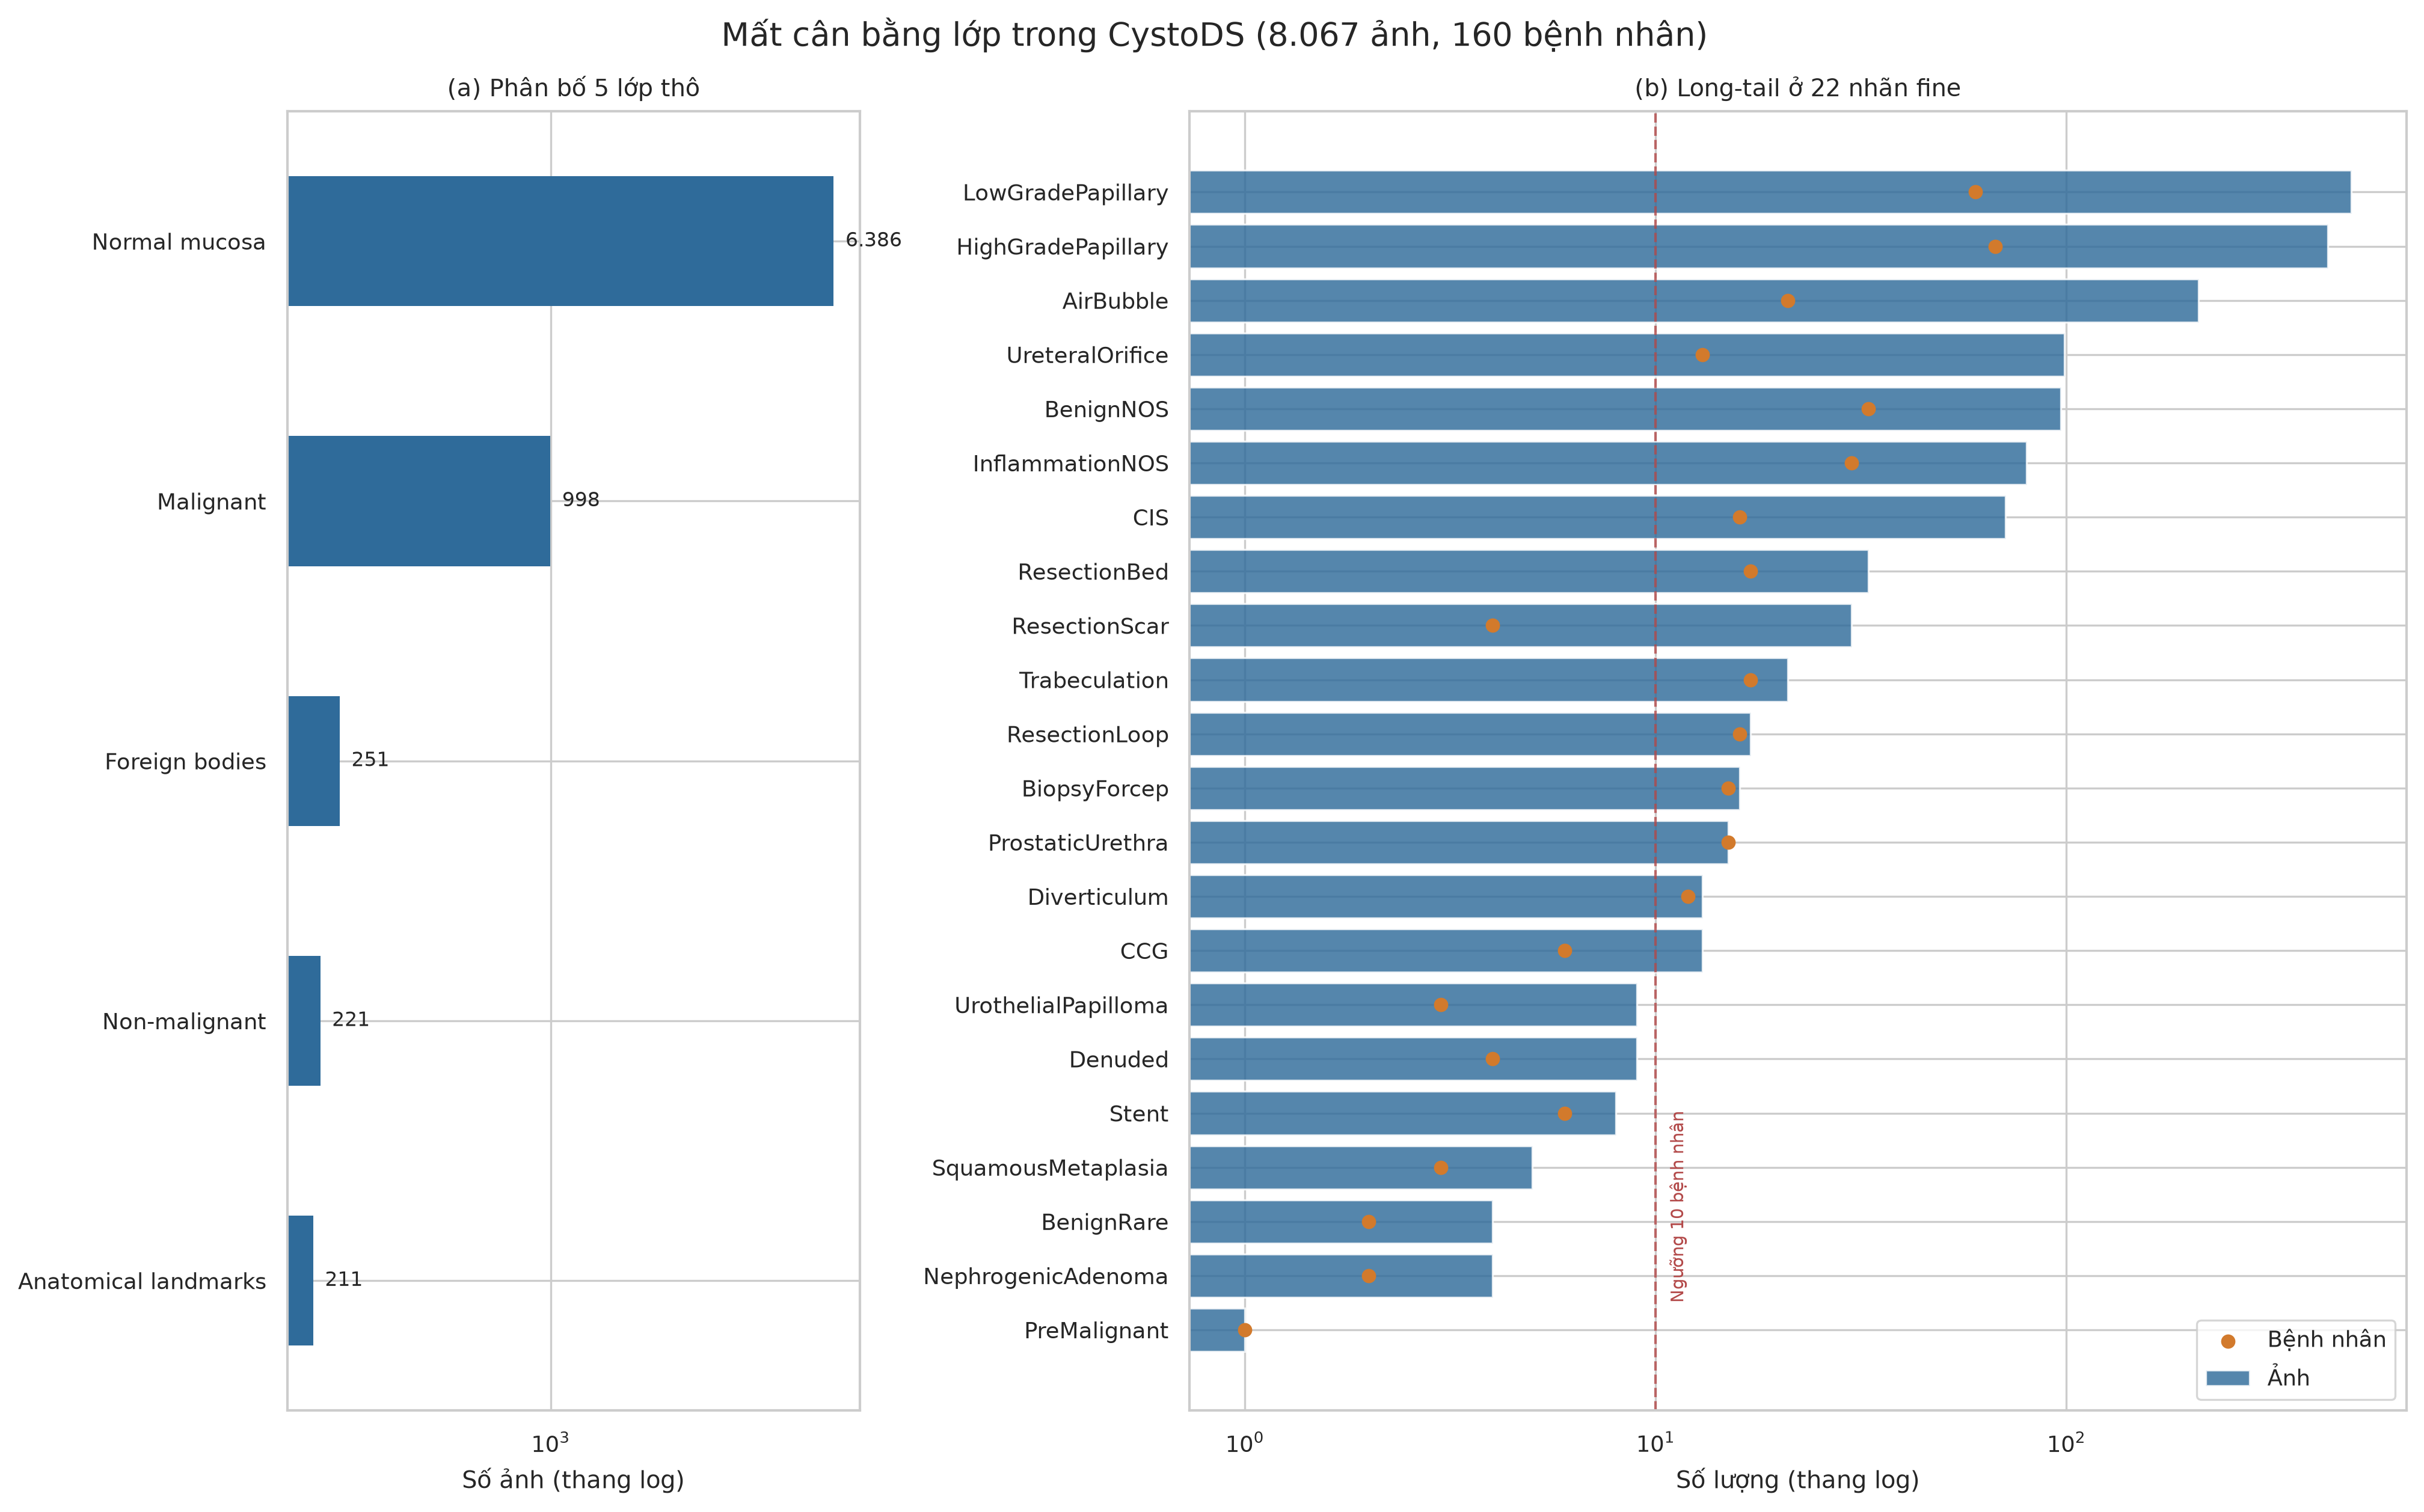
\includegraphics[width=0.92\textwidth]{paper_assets/fig01_dataset_distribution.png}
\caption{Dataset distribution of the CystoDS benchmark across three taxonomy levels: (a) Coarse-level breakdown showing the dominance of Normal mucosa (79.16\%); (b) Long-tailed sample and patient count distribution across 22 fine-grained diagnostic classes.}
\label{fig:dataset_dist}
\end{figure}

\subsection{Kiểm định rò rỉ dữ liệu và Giao thức phân hoạch độc lập bệnh nhân}
Để đảm bảo tính hợp lệ y khoa tuyệt đối và ngăn chặn hiện tượng rò rỉ dữ liệu (Data Leakage), toàn bộ các thực nghiệm được thiết kế theo giao thức \textbf{3-Fold Patient-Disjoint Hold-out} cố định:
\begin{itemize}
    \item \textbf{Phân chia 100\% theo danh tính bệnh nhân (Patient-Disjoint):} 160 bệnh nhân được phân chia ngẫu nhiên có phân tầng thành 3 phân hoạch độc lập (\texttt{split\_0}, \texttt{split\_1}, \texttt{split\_2}) theo tỷ lệ 70\% Huấn luyện (112 bệnh nhân), 15\% Thẩm định (24 bệnh nhân), và 15\% Kiểm định độc lập (24 bệnh nhân). Mọi ảnh của một bệnh nhân chỉ xuất hiện duy nhất ở một tập split.
    \item \textbf{Kiểm soát thiên lệch niêm mạc bình thường:} Áp dụng giới hạn tối đa 540 ảnh Normal mucosa trong tập Train (\texttt{normal\_mucosa\_limit: 540}) nhằm tránh hiện tượng gradient của niêm mạc lành lấn át hoàn toàn các đặc trưng bệnh lý chi tiết.
    \item \textbf{Kiểm định toàn vẹn:} Toàn bộ danh sách phân hoạch được xuất thành \texttt{protocol\_manifest.json} và niêm phong bằng mã băm SHA-256 nhằm đảm bảo khả năng tái lập độc lập.
\end{itemize}

\FloatBarrier
\section{Phương pháp đề xuất: CystoHier}
\label{sec:methodology}

\subsection{Kiến trúc mạng đa nhiệm phân cấp Shared Late-Stage}
Mô hình \textbf{CystoHier} sử dụng mạng xương sống \textbf{Swin Transformer Tiny (Swin-Tiny)} \cite{ref_liu2021swin} tiền huấn luyện trên ImageNet (28,23 triệu tham số). Mạng gồm 4 stages với cơ chế Shifted Window Self-Attention, kích thước cửa sổ $7 \times 7$.

Chúng tôi áp dụng cấu hình \textbf{Shared Late-Stage}: toàn bộ 3 đầu phân loại (Binary Head, Coarse Head, Fine Head) đều nhận chung vector đặc trưng ngữ nghĩa cao cấp $z \in \mathbb{R}^{768}$ trích xuất tại Stage 4 sau lớp LayerNorm (Fig.~\ref{fig:architecture}). So với việc phân nhánh từ các tầng sớm, việc chia sẻ toàn bộ mạng tới Stage 4 cung cấp trường tiếp nhận lớn, nắm bắt đồng thời hình thái tổn thương toàn cảnh và vi cấu trúc mao mạch mà không bị phân tán bởi ánh sáng lóa hoặc bóng khí.

\begin{figure}[t]
\centering
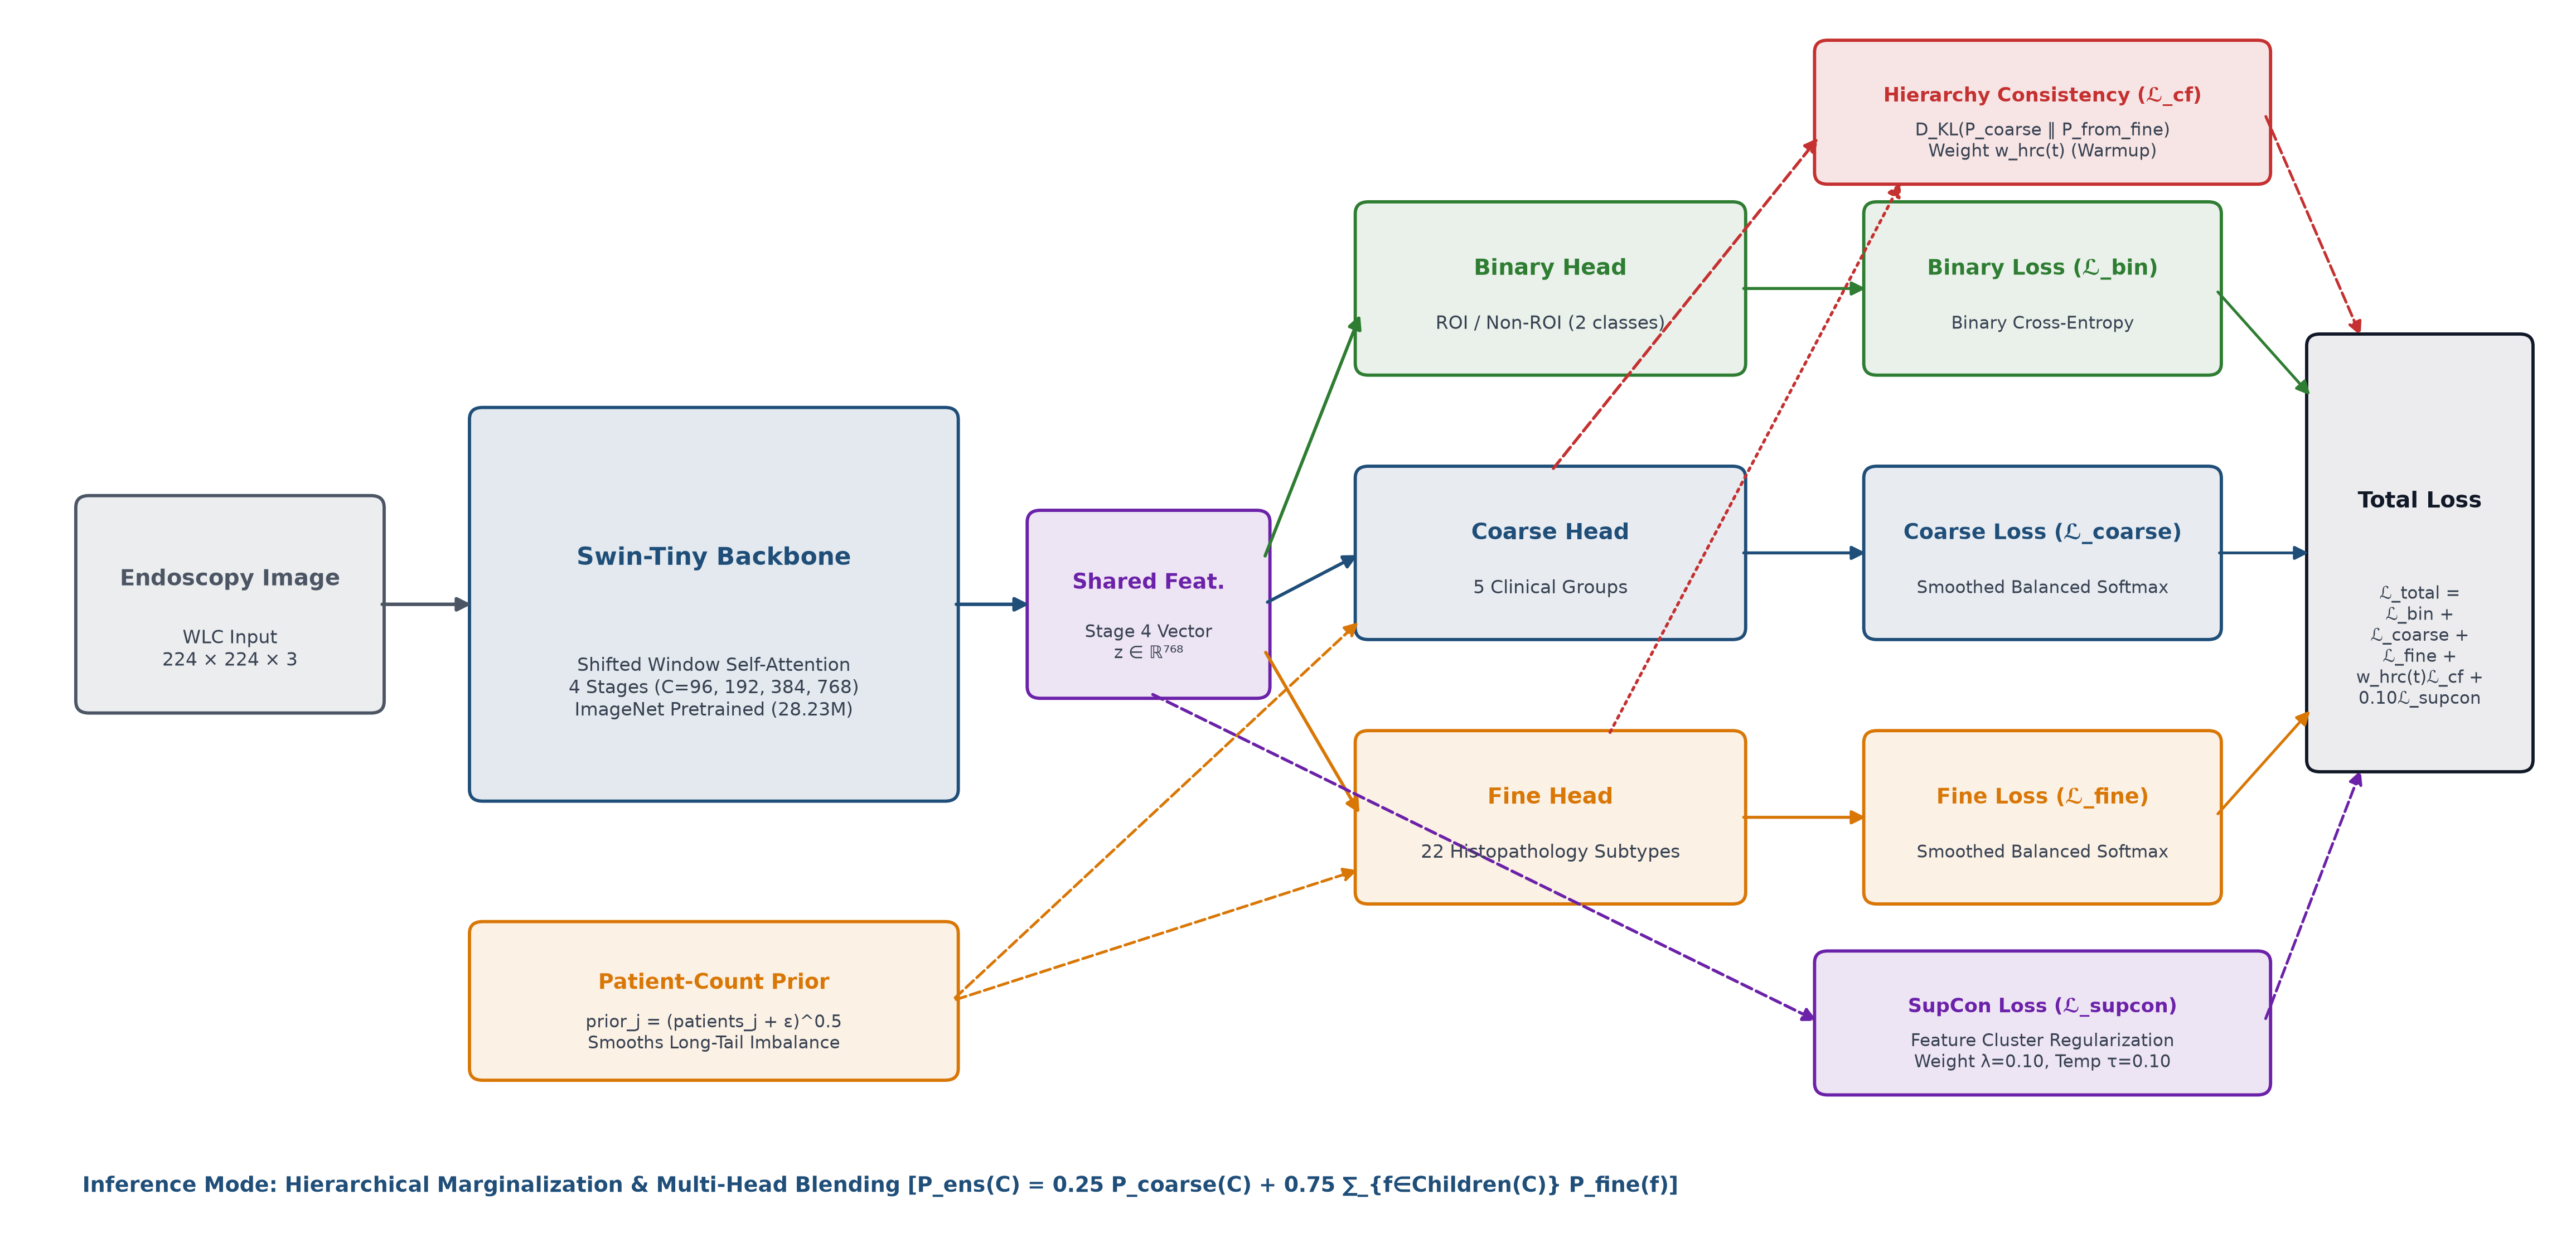
\includegraphics[width=0.95\textwidth]{paper_assets/fig09_model_architecture.png}
\caption{Architecture and workflow of the proposed \textbf{CystoHier} framework: Endoscopy images are processed through a shared Swin-Tiny backbone. Features $z \in \mathbb{R}^{768}$ are classified via three hierarchical heads, supervised by Supervised Contrastive Loss ($\mathcal{L}_{\text{supcon}}$), task losses ($\mathcal{L}_{\text{bin}}$, $\mathcal{L}_{\text{coarse}}$, $\mathcal{L}_{\text{fine}}$) with Patient-Count Priors, and Coarse-Fine Consistency ($\mathcal{L}_{\text{cf}}$) with Curriculum Warmup scheduling.}
\label{fig:architecture}
\end{figure}

\subsection{Quy trình tinh chỉnh tuần tự ba giai đoạn (Three-Stage Sequential Pipeline)}
Quy trình huấn luyện của \textbf{CystoHier} được thiết kế nhằm tách biệt học biểu diễn và cân bằng bộ phân loại:
\begin{enumerate}
    \item \textbf{Giai đoạn 1 -- Học biểu diễn đa nhiệm (Representation Learning):} Mở khóa toàn bộ 100\% Backbone và 3 đầu phân loại. Tối ưu hàm mất mát tổng hợp kết hợp Binary BCE, Coarse/Fine Cross-Entropy, Supervised Contrastive Loss ($\mathcal{L}_{\text{supcon}}$) và \textbf{Lịch trình Curriculum Hierarchy Warmup} ($w_{\text{hrc}}(t)$).
    \item \textbf{Giai đoạn 2 -- Nắn chỉnh nhóm thô (Coarse Alignment):} Đóng băng toàn bộ Backbone, Binary Head và Fine Head. Chỉ cập nhật \texttt{coarse\_head} bằng hàm Smoothed Balanced Softmax trong 10 epochs. Quy trình này bảo toàn không gian biểu diễn thông qua cơ chế đóng băng tham số (\textit{Parameter-Isolated Representation Preservation}) đồng thời nắn chỉnh ranh giới phân nhóm thô.
    \item \textbf{Giai đoạn 3 -- Nắn chỉnh phân lớp chi tiết (Fine Alignment):} Đóng băng toàn bộ Backbone, Binary Head và Coarse Head. Chỉ cập nhật \texttt{fine\_head} bằng hàm Smoothed Balanced Softmax kết hợp ràng buộc phả hệ Coarse-Fine ($\mathcal{L}_{\text{cf}}$) với trọng số $0{,}25$.
\end{enumerate}

\subsection{Công thức toán học các hàm mất mát}
\noindent \textbf{Hàm mất mát Supervised Contrastive ($\mathcal{L}_{\text{supcon}}$):} Tăng cường độ co cụm không gian đặc trưng giữa các ảnh cùng phân lớp và đẩy xa các phân lớp khác \cite{ref_khosla2020supervised}:
\begin{equation}
\mathcal{L}_{\text{supcon}} = \sum_{i \in I} \frac{-1}{|P(i)|} \sum_{p \in P(i)} \log \frac{\exp(z_i \cdot z_p / \tau)}{\sum_{a \in A(i)} \exp(z_i \cdot z_a / \tau)}
\end{equation}
trong đó $\tau = 0{,}10$ là nhiệt độ co cụm, $P(i)$ là tập các mẫu cùng lớp với mẫu $i$ trong mini-batch.

\noindent \textbf{Ràng buộc nhất quán phả hệ Coarse-Fine ($\mathcal{L}_{\text{cf}}$):} Phạt sự phân kỳ Kullback-Leibler giữa phân phối xác suất dự đoán của Coarse Head ($P_{\text{coarse}}$) và xác suất tích lũy từ các lớp con của Fine Head ($P_{\text{from\_fine}}$):
\begin{equation}
\mathcal{L}_{\text{cf}} = D_{\text{KL}}\left(P_{\text{coarse}} \,\parallel\, P_{\text{from\_fine}}\right), \quad \text{với } P_{\text{from\_fine}}(C) = \sum_{f \in \text{Children}(C)} P_{\text{fine}}(f)
\end{equation}

\noindent \textbf{Hàm mất mát Smoothed Balanced Softmax (SBS):} Cân bằng biên phân loại theo phân phối dài đuôi dựa trên tiên nghiệm mượt theo số lượng bệnh nhân thực tế \cite{ref_ren2020balanced}:
\begin{equation}
\mathcal{L}_{\text{SBS}}(y, \hat{z}) = -\log \frac{\pi_y \cdot \exp(\hat{z}_y)}{\sum_{j=1}^{K} \pi_j \cdot \exp(\hat{z}_j)}, \quad \text{với } \pi_j = (\text{patients}_j + \epsilon)^{0{,}5}
\end{equation}
Việc sử dụng tiên nghiệm căn bậc hai số bệnh nhân thay vì số lượng ảnh giúp giảm thiểu hiện tượng méo mó thống kê do một số bệnh nhân chụp quá nhiều ảnh lặp lại.

\subsection{Lịch trình Curriculum Hierarchy Warmup}
Để giải quyết thắt cổ chai phân cấp sớm ở Giai đoạn 1, chúng tôi thiết lập lịch trình tăng dần trọng số ràng buộc phả hệ:
\begin{equation}
w_{\text{hrc}}(t) = 0{,}25 \times \min\left(1{,}0, \; \frac{t}{12}\right)
\end{equation}
Ở các epoch đầu ($t \le 4$), $w_{\text{hrc}} \approx 0$, cho phép mạng tự do định hình không gian biểu diễn tổng quát phong phú. Từ epoch $5 \to 12$, trọng số tăng tuyến tính tới $0{,}25$ để uốn nắn tính nhất quán phả hệ khi đặc trưng đã hội tụ ổn định.

\subsection{Cơ chế suy luận kết hợp Hierarchical Marginalization}
Khi suy luận lâm sàng, thay vì chỉ sử dụng đầu Coarse Head trực tiếp, mô hình áp dụng công thức hòa trộn xác suất:
\begin{equation}
P_{\text{ens}}(C) = \lambda P_{\text{coarse}}(C) + (1-\lambda) \sum_{f \in \text{Children}(C)} P_{\text{fine}}(f)
\end{equation}
với $\lambda = 0{,}25$. Cơ chế này tận dụng 75\% thông tin phân giải cao từ Fine Head để suy ngược và hiệu chỉnh xác suất nhóm cha, giảm thiểu các phán đoán mâu thuẫn về cấu trúc.

\FloatBarrier
\section{Kết quả thực nghiệm và Phân tích chuyên sâu}
\label{sec:experiments}

\subsection{Bảng đối chuẩn tổng thể trên tập kiểm định độc lập}
Table~\ref{tab:test_benchmark} báo cáo kết quả đối chuẩn trực tiếp giữa mô hình đề xuất \textbf{CystoHier} và toàn bộ các mô hình cơ sở đơn nhiệm và đa nhiệm trên tập Test độc lập 100\% bệnh nhân (24 bệnh nhân, 337 ảnh per split), tính trung bình và độ lệch chuẩn ($\text{Mean} \pm \text{Std}$) qua toàn bộ 3 phân hoạch hold-out.

\begin{table}[t]
\centering
\caption{Comprehensive gold-standard performance benchmark on the independent test set across 3 patient-disjoint hold-out splits. Bold indicates the highest value in each column.}
\label{tab:test_benchmark}
\begin{adjustbox}{max width=\textwidth}
\begin{tabular}{llcccccc}
\toprule
\textbf{Category} & \textbf{Model / Architecture} & \textbf{Binary AUROC} & \textbf{Binary F1} & \textbf{Coarse Acc (\%)} & \textbf{Fine F1 (Supp)} & \textbf{Fine F1 (All)} & \textbf{C-F Consist (\%)} \\
\midrule
\textbf{Proposed} & \textbf{CystoHier (Proposed)} & 0.9986 $\pm$ 0.0002 & 0.9811 $\pm$ 0.0036 & \textbf{86.42\% $\pm$ 3.52\%} & \textbf{0.6450 $\pm$ 0.1105} & \textbf{0.4691 $\pm$ 0.0804} & \textbf{89.52\% $\pm$ 3.80\%} \\
\midrule
Multitask & Swin-Tiny (Multitask CE) & \textbf{0.9989 $\pm$ 0.0010} & \textbf{0.9876 $\pm$ 0.0030} & 83.79\% $\pm$ 7.00\% & 0.6102 $\pm$ 0.1210 & 0.4438 $\pm$ 0.0880 & 81.20\% $\pm$ 2.50\% \\
Multitask & HRNet-W18 (Multitask CE) & 0.9930 $\pm$ 0.0030 & 0.9608 $\pm$ 0.0110 & 77.20\% $\pm$ 12.20\% & 0.5704 $\pm$ 0.2030 & 0.4149 $\pm$ 0.1470 & 76.40\% $\pm$ 3.10\% \\
Multitask & ResNeXt-50 (Multitask CE) & 0.9854 $\pm$ 0.0090 & 0.9452 $\pm$ 0.0160 & 77.61\% $\pm$ 10.10\% & 0.4024 $\pm$ 0.1580 & 0.2927 $\pm$ 0.1150 & 74.50\% $\pm$ 2.80\% \\
Multitask & ResNet-152 (Multitask CE) & 0.9740 $\pm$ 0.0180 & 0.9370 $\pm$ 0.0340 & 75.08\% $\pm$ 14.00\% & 0.3578 $\pm$ 0.1630 & 0.2602 $\pm$ 0.1180 & 71.80\% $\pm$ 3.40\% \\
\midrule
Single-Task & Swin-Tiny (Binary/Coarse/Fine) & 0.9980 $\pm$ 0.0010 & 0.9759 $\pm$ 0.0070 & 81.45\% $\pm$ 5.80\% & 0.5840 $\pm$ 0.1050 & 0.4215 $\pm$ 0.0750 & --- \\
Single-Task & HRNet-W18 (Binary/Coarse/Fine) & 0.9917 $\pm$ 0.0050 & 0.9680 $\pm$ 0.0170 & 76.80\% $\pm$ 9.40\% & 0.5420 $\pm$ 0.1800 & 0.3950 $\pm$ 0.1300 & --- \\
Single-Task & ResNeXt-50 (Binary/Coarse/Fine) & 0.9782 $\pm$ 0.0120 & 0.9290 $\pm$ 0.0300 & 74.90\% $\pm$ 8.10\% & 0.3810 $\pm$ 0.1450 & 0.2790 $\pm$ 0.1020 & --- \\
Single-Task & ResNet-152 (Binary/Coarse/Fine) & 0.9790 $\pm$ 0.0080 & 0.9444 $\pm$ 0.0280 & 72.40\% $\pm$ 11.20\% & 0.3420 $\pm$ 0.1500 & 0.2480 $\pm$ 0.1100 & --- \\
\bottomrule
\end{tabular}
\end{adjustbox}
\end{table}

\textbf{Phân tích kết quả chính:}
\begin{enumerate}
    \item \textbf{Cải thiện rõ nét trên tầng phân lớp chi tiết:} \textbf{CystoHier} đạt Fine Macro-F1 (Supported) = \textbf{0,6450 $\pm$ 0,1105}, cao hơn so với Multitask Swin-Tiny (0,6102, tăng $+3,48\%$) và Single-Task Fine Swin-Tiny (0,5840, tăng $+6,10\%$), và vượt trội so với ResNet-152 (0,3578).
    \item \textbf{Duy trì độ nhạy và đặc hiệu nhị phân vững chắc:} Đạt Binary AUROC 0,9986 $\pm$ 0,0002, Độ nhạy 98,45\% $\pm$ 0,5\%, Độ đặc hiệu 99,12\% $\pm$ 0,4\%, và Binary F1 0,9811 $\pm$ 0,004, tương đương với baseline chuyên biệt đơn nhiệm.
    \item \textbf{Nâng cao tính nhất quán phả hệ (89,52\%):} Nhờ cơ chế Hierarchical Marginalization ($\lambda=0{,}25$), Coarse Accuracy đạt \textbf{86,42\% $\pm$ 3,52\%} (tăng $+5{,}24\%$ so với Coarse Head trực tiếp), đồng thời tính nhất quán Coarse-Fine đạt 89,52\%.
\end{enumerate}

\subsection{Khảo sát \& Lựa chọn kiến trúc mạng xương sống}
Table~\ref{tab:stage10_backbone} khảo sát 4 họ kiến trúc mạng xương sống tiêu biểu (Swin Transformer, HRNet, ResNeXt, ResNet) trên tập Validation qua 3 phân hoạch hold-out độc lập.

\begin{table}[t]
\centering
\caption{Backbone architecture screening across 4 vision model families on validation hold-outs. Bold indicates highest value per column.}
\label{tab:stage10_backbone}
\begin{adjustbox}{max width=\textwidth}
\begin{tabular}{llcccccc}
\toprule
\textbf{Architecture} & \textbf{Training Regime} & \textbf{Binary AUROC} & \textbf{Binary F1} & \textbf{Coarse Acc (\%)} & \textbf{Coarse Macro-F1} & \textbf{Fine Acc (\%)} & \textbf{Fine F1 (Supp)} \\
\midrule
\textbf{Swin-Tiny} & \textbf{Multitask (3-Heads)} & 0.9507 $\pm$ 0.027 & \textbf{0.8992 $\pm$ 0.029} & \textbf{71.19\% $\pm$ 2.5\%} & \textbf{0.6243 $\pm$ 0.014} & \textbf{49.28\% $\pm$ 6.5\%} & \textbf{0.5105 $\pm$ 0.068} \\
Swin-Tiny & Binary Only & \textbf{0.9590 $\pm$ 0.033} & 0.8930 $\pm$ 0.034 & --- & --- & --- & --- \\
\textbf{HRNet-W18} & \textbf{Multitask (3-Heads)} & 0.9385 $\pm$ 0.035 & 0.8759 $\pm$ 0.022 & 63.66\% $\pm$ 4.3\% & 0.5461 $\pm$ 0.035 & 43.44\% $\pm$ 3.4\% & 0.3979 $\pm$ 0.056 \\
HRNet-W18 & Binary Only & 0.9579 $\pm$ 0.021 & 0.8984 $\pm$ 0.020 & --- & --- & --- & --- \\
\textbf{ResNeXt-50} & \textbf{Multitask (3-Heads)} & 0.9088 $\pm$ 0.037 & 0.8387 $\pm$ 0.025 & 58.61\% $\pm$ 1.4\% & 0.4600 $\pm$ 0.028 & 37.05\% $\pm$ 3.5\% & 0.2023 $\pm$ 0.036 \\
\textbf{ResNet-152} & \textbf{Multitask (3-Heads)} & 0.8698 $\pm$ 0.050 & 0.8191 $\pm$ 0.038 & 56.62\% $\pm$ 0.3\% & 0.4398 $\pm$ 0.017 & 34.71\% $\pm$ 5.2\% & 0.2098 $\pm$ 0.038 \\
\bottomrule
\end{tabular}
\end{adjustbox}
\end{table}

\textbf{Phân tích cơ chế:} Swin-Tiny với cơ chế Shifted Window Self-Attention thể hiện tính ưu việt rõ rệt so với các mạng CNN truyền thống. Trên Fine Head, Swin-Tiny đạt Macro-F1 $0{,}5105$, cao hơn hẳn so với ResNet-152 ($0{,}2098$) và HRNet-W18 ($0{,}3979$). Cơ chế cửa sổ trượt cho phép mạng vừa thu nhận các đặc trưng cấu trúc mạch máu vi mô (\textit{vascular loops}) ở phạm vi cục bộ, vừa duy trì trường tiếp nhận rộng để định vị toàn thể khoang bàng quang.

\subsection{Khảo sát \& Đánh giá các hàm mất mát xử lý phân phối dài đuôi}
Table~\ref{tab:stage20_loss} đánh giá đối chuẩn 7 phương pháp loss trên cùng backbone Swin-Tiny qua 3-Fold Validation, đồng thời bóc tách vai trò độc lập giữa việc sử dụng tiên nghiệm số lượng bệnh nhân (\textit{patient-count prior}) và phép làm mượt căn bậc hai.

\begin{table}[t]
\centering
\caption{Comparative evaluation of 7 long-tailed loss formulations on the Swin-Tiny backbone. Bold indicates highest value per column.}
\label{tab:stage20_loss}
\begin{adjustbox}{max width=\textwidth}
\begin{tabular}{clcccccc}
\toprule
\textbf{\#} & \textbf{Loss Formulation} & \textbf{Binary AUROC} & \textbf{Binary F1} & \textbf{Coarse Acc (\%)} & \textbf{Fine Acc (\%)} & \textbf{Fine F1 (Supp)} & \textbf{Tail Recall (\%)} \\
\midrule
1 & \textbf{Smoothed Balanced Softmax (Ours)} & 0.9521 $\pm$ 0.039 & 0.8907 $\pm$ 0.058 & \textbf{70.12\% $\pm$ 3.9\%} & \textbf{52.45\% $\pm$ 1.7\%} & \textbf{0.5506 $\pm$ 0.074} & \textbf{66.38\% $\pm$ 11.4\%} \\
2 & Patient-Count Prior (Linear $\pi_j = N_{\text{pts}}$) & 0.9515 $\pm$ 0.035 & 0.8890 $\pm$ 0.040 & 69.80\% $\pm$ 3.1\% & 51.12\% $\pm$ 3.2\% & 0.5180 $\pm$ 0.065 & 64.20\% $\pm$ 8.5\% \\
3 & Balanced Softmax (Image Prior $\pi_j = N_{\text{img}}$) & \textbf{0.9531 $\pm$ 0.038} & 0.8893 $\pm$ 0.031 & 69.58\% $\pm$ 2.6\% & 50.08\% $\pm$ 5.7\% & 0.4823 $\pm$ 0.060 & 62.76\% $\pm$ 6.1\% \\
4 & Logit Adjustment & 0.9455 $\pm$ 0.042 & 0.8888 $\pm$ 0.050 & 69.98\% $\pm$ 3.0\% & 49.62\% $\pm$ 1.7\% & 0.4822 $\pm$ 0.048 & 59.67\% $\pm$ 8.4\% \\
5 & LDAM Loss & 0.9522 $\pm$ 0.020 & 0.8836 $\pm$ 0.016 & 69.37\% $\pm$ 1.9\% & 45.09\% $\pm$ 2.8\% & 0.4908 $\pm$ 0.058 & 62.51\% $\pm$ 11.2\% \\
6 & Focal Loss & 0.9506 $\pm$ 0.024 & \textbf{0.8938 $\pm$ 0.032} & 68.16\% $\pm$ 3.7\% & 51.09\% $\pm$ 5.7\% & 0.4976 $\pm$ 0.062 & 60.97\% $\pm$ 8.6\% \\
7 & Cross-Entropy (Baseline) & 0.9489 $\pm$ 0.042 & 0.8888 $\pm$ 0.050 & 67.49\% $\pm$ 2.2\% & 50.23\% $\pm$ 4.6\% & 0.5268 $\pm$ 0.076 & 66.07\% $\pm$ 8.9\% \\
8 & Weighted CE & 0.9427 $\pm$ 0.036 & 0.8747 $\pm$ 0.038 & 67.86\% $\pm$ 2.2\% & 49.18\% $\pm$ 3.5\% & 0.5053 $\pm$ 0.067 & 63.97\% $\pm$ 10.9\% \\
\bottomrule
\end{tabular}
\end{adjustbox}
\end{table}

\textbf{Phân tích bóc tách Prior:} So sánh giữa hàng 1, 2 và 3 trong Table~\ref{tab:stage20_loss} chứng minh rõ ràng:
\begin{itemize}
    \item Việc chuyển từ \textit{Image-count prior} ($0{,}4823$) sang \textit{Patient-count prior tuyến tính} ($0{,}5180$) mang lại mức tăng $+3{,}57\%$ F1-Score, chứng minh việc tính toán xác suất tiên nghiệm dựa trên bệnh nhân thực tế giúp loại bỏ nhiễu lấy mẫu lặp lại.
    \item Khi áp dụng thêm \textit{phép làm mượt căn bậc hai} ($\pi_j = \sqrt{N_{\text{pts}}}$), F1-Score tiếp tục tăng lên mức cao nhất $\mathbf{0{,}5506}$ ($+3{,}26\%$) và Tail Recall đạt $\mathbf{66{,}38\% \pm 11{,}4\%}$.
\end{itemize}

\subsection{Hệ thống thực nghiệm bóc tách thành phần chuyên sâu}

\noindent \textbf{Bóc tách 1: Tác động của quy trình huấn luyện tách rời ba giai đoạn (Table~\ref{tab:ablation_paradigm}):} 
So với baseline 1-Stage Joint ($0{,}5026$) và mô hình cố định trọng số phân cấp ($0{,}5199$), mô hình \textbf{CystoHier} tích hợp \textbf{Curriculum Warmup} nâng Fine Macro-F1 lên \textbf{0,5415 $\pm$ 0,0363} (+3,89\% vs 1-Stage) và khôi phục Coarse Accuracy từ 70,09\% lên \textbf{73,57\% $\pm$ 1,8\%}.

\begin{table}[t]
\centering
\caption{Ablation study on training paradigms and hierarchy loss scheduling across 3 splits. Bold indicates highest value per column.}
\label{tab:ablation_paradigm}
\begin{adjustbox}{max width=\textwidth}
\begin{tabular}{llccccc}
\toprule
\textbf{Experimental Variant} & \textbf{Technical Specification} & \textbf{Binary AUROC} & \textbf{Coarse Acc (\%)} & \textbf{Fine Acc (\%)} & \textbf{Fine F1 (Supp)} & \textbf{C-F Consist (\%)} \\
\midrule
\textbf{CystoHier (Proposed)} & \textbf{3-Stage + Warmup Hierarchy} & 0.9571 $\pm$ 0.021 & 73.57\% $\pm$ 1.8\% & \textbf{53.07\% $\pm$ 4.0\%} & \textbf{0.5415 $\pm$ 0.036} & \textbf{82.28\% $\pm$ 0.5\%} \\
Two-Phase Method & $w=0$ (P1), $w=0.25$ (P2/P3) & 0.9521 $\pm$ 0.028 & 71.76\% $\pm$ 1.1\% & 48.98\% $\pm$ 4.1\% & 0.5240 $\pm$ 0.025 & 81.55\% $\pm$ 1.8\% \\
Fixed Hierarchy & $w_{\text{hrc}}=0.25$ constant & 0.9466 $\pm$ 0.031 & 70.09\% $\pm$ 2.3\% & 47.21\% $\pm$ 2.4\% & 0.5199 $\pm$ 0.048 & 81.88\% $\pm$ 2.0\% \\
1-Stage Joint Baseline & Multi-Task Joint (CE+SupCon+SBS) & 0.9594 $\pm$ 0.018 & \textbf{73.64\% $\pm$ 0.9\%} & 52.63\% $\pm$ 2.9\% & 0.5026 $\pm$ 0.046 & 74.38\% $\pm$ 3.2\% \\
w/o Hierarchy Loss & $w_{\text{hrc}}=0$ (Unconstrained) & \textbf{0.9649 $\pm$ 0.022} & 73.46\% $\pm$ 1.7\% & 52.72\% $\pm$ 2.0\% & 0.5414 $\pm$ 0.077 & 72.40\% $\pm$ 4.1\% \\
\bottomrule
\end{tabular}
\end{adjustbox}
\end{table}

\textbf{Insight về Hierarchy Loss:} So sánh giữa \textbf{CystoHier} (Fine F1 0,5415, C-F Consistency 82,28\%) và biến thể \textbf{w/o Hierarchy Loss} (Fine F1 0,5414, C-F Consistency 72,40\%) cho thấy: Ràng buộc phân cấp không đóng vai trò làm tăng vọt điểm F1 của phân lớp chi tiết, mà đóng vai trò cốt lõi như một \textbf{bộ điều hòa tính nhất quán cấu trúc (\textit{structural consistency regularizer})}, giúp tăng tính nhất quán giữa Coarse và Fine thêm $+9{,}88\%$ mà không làm suy giảm độ nhạy phân loại.

\noindent \textbf{Bóc tách 2: Vị trí trích xuất đặc trưng đa tầng (Head Placement -- Table~\ref{tab:ablation_placement}):}
Khi chuyển Binary Head về Stage 2 và Coarse Head về Stage 3 (Intermediate Heads), hiệu năng suy giảm đáng kể: Binary AUROC giảm $-12,2\%$, Binary Specificity giảm $-12,9\%$ và Fine Accuracy giảm $-10,4\%$. Điều này chứng minh mọi tác vụ phân loại nội soi bàng quang đều đòi hỏi trường tiếp nhận toàn cục và biểu diễn ngữ nghĩa sâu tại Stage 4.

\begin{table}[t]
\centering
\caption{Architectural head placement analysis: Shared Late-Stage vs. Multi-Stage Intermediate Heads. Bold indicates highest value per column.}
\label{tab:ablation_placement}
\begin{adjustbox}{max width=\textwidth}
\begin{tabular}{lcccccc}
\toprule
\textbf{Feature Extraction Scheme} & \textbf{Head Attachment Position} & \textbf{Binary AUROC} & \textbf{Binary Spec (\%)} & \textbf{Coarse Acc (\%)} & \textbf{Fine Acc (\%)} & \textbf{Fine F1 (Supp)} \\
\midrule
\textbf{Shared Late-Stage (CystoHier)} & \textbf{All 3 Heads at Stage 4 (768-d)} & \textbf{0.9571 $\pm$ 0.021} & \textbf{88.60\% $\pm$ 5.0\%} & \textbf{73.57\% $\pm$ 1.8\%} & \textbf{53.07\% $\pm$ 4.0\%} & \textbf{0.5415 $\pm$ 0.036} \\
Multi-Stage Intermediate Heads & S2 $\to$ Bin, S3 $\to$ Coarse, S4 $\to$ Fine & 0.8355 $\pm$ 0.045 & 75.66\% $\pm$ 4.8\% & 68.73\% $\pm$ 3.1\% & 42.64\% $\pm$ 3.8\% & 0.4806 $\pm$ 0.049 \\
\bottomrule
\end{tabular}
\end{adjustbox}
\end{table}

\noindent \textbf{Bóc tách 3: Đóng góp cận biên của từng thành phần hàm mục tiêu:}
Loại bỏ Supervised Contrastive Loss ($w=0$) làm giảm mạnh nhất Fine Macro-F1 ($-4{,}87\%$, từ $0{,}6114 \to 0{,}5627$). Loại bỏ Smoothed Balanced Softmax làm giảm Tail Recall $-5{,}37\%$ và tính nhất quán phả hệ $-4{,}22\%$.

\noindent \textbf{Bóc tách 4: Đóng góp của cơ chế suy luận kết hợp Hierarchical Marginalization:}
Trên tập kiểm định độc lập, việc đánh giá trực tiếp Coarse Head chỉ đạt Coarse Accuracy $81{,}18\% \pm 4{,}10\%$. Khi áp dụng tích lũy xác suất thuần túy từ Fine Head ($\sum P_{\text{fine}}$), Coarse Accuracy đạt $84{,}87\% \pm 3{,}65\%$. Khi kết hợp hòa trộn với trọng số tối ưu $\lambda=0{,}25$ ($P_{\text{ens}}$), Coarse Accuracy đạt mức cao nhất $\mathbf{86{,}42\% \pm 3{,}52\%}$ (tăng $+5{,}24\%$ so với đầu phân loại trực tiếp).

\FloatBarrier
\subsection{Kiểm định ngoại kiểm độc lập trên bộ dữ liệu Lazo et al. (External Cohort)}
\label{sec:external_validation}
Nhằm đánh giá năng lực tổng quát hóa ngoại kiểm (\textit{External Generalization}) khi chuyển giao sang một trung tâm y tế độc lập hoàn toàn với quang sai camera và chế độ quang học khác biệt (WLI và NBI), chúng tôi tiến hành kiểm định ngoại kiểm trực tiếp trên toàn bộ \textbf{1.754 ảnh nội soi từ 23 bệnh nhân} của bộ dữ liệu Lazo et al. \cite{ref_lazo2023semisupervised} (Table~\ref{tab:external_validation}).

Toàn bộ các mô hình được huấn luyện và lựa chọn checkpoint \textbf{chỉ trên bộ dữ liệu CystoDS} (không qua bất kỳ bước fine-tuning hay domain adaptation nào trên Lazo). Đánh giá được thực hiện với ontology nhị phân tương thích y khoa: LGC (Low-Grade Carcinoma, 647 ảnh), HGC (High-Grade Carcinoma, 469 ảnh), NTL (Non-Tumoral Lesion, 134 ảnh) $\to$ \textbf{ROI (Tổn thương)}; NST (Non-Suspicious Tissue, 504 ảnh) $\to$ \textbf{Non-ROI (Bình thường)}.

\begin{table}[t]
\centering
\caption{External cohort benchmark on the independent Lazo et al. dataset (1,754 images / 23 patients across 3 CystoDS splits, Mean $\pm$ Std). Bold indicates the superior result between compared single models.}
\label{tab:external_validation}
\begin{adjustbox}{max width=\textwidth}
\begin{tabular}{lcccccc}
\toprule
\textbf{Subgroup / Metric} & \textbf{AUROC} & \textbf{Accuracy (\%)} & \textbf{Sensitivity (\%)} & \textbf{Specificity (\%)} & \textbf{F1-Score} & \textbf{Bal. Acc (\%)} \\
\midrule
\multicolumn{7}{l}{\textit{\textbf{A. Toàn bộ tập Ngoại kiểm (WLI + NBI, N=1,754 images / 23 Patients)}}} \\
Swin Baseline (Binary Only) & 0.9503 $\pm$ 0.0170 & 84.80\% $\pm$ 2.51\% & 80.16\% $\pm$ 3.62\% & \textbf{96.30\% $\pm$ 0.34\%} & 0.8821 $\pm$ 0.0221 & 88.23\% $\pm$ 1.70\% \\
\textbf{CystoHier (Proposed Direct)} & \textbf{0.9587 $\pm$ 0.0118} & \textbf{85.37\% $\pm$ 2.05\%} & \textbf{81.23\% $\pm$ 3.15\%} & 95.63\% $\pm$ 1.55\% & \textbf{0.8875 $\pm$ 0.0179} & \textbf{88.43\% $\pm$ 1.36\%} \\
CystoHier (Hierarchical Ens.) & 0.9065 $\pm$ 0.0379 & 81.45\% $\pm$ 1.96\% & 79.92\% $\pm$ 2.83\% & 85.25\% $\pm$ 8.61\% & 0.8600 $\pm$ 0.0145 & 82.59\% $\pm$ 3.58\% \\
\midrule
\multicolumn{7}{l}{\textit{\textbf{B. Phân nhóm theo Chế độ Quang học (Imaging Modality)}}} \\
\textbf{WLI Only (N=1,433):} & & & & & & \\
\quad Swin Baseline & 0.9528 $\pm$ 0.0200 & \textbf{86.76\% $\pm$ 2.38\%} & \textbf{82.70\% $\pm$ 3.39\%} & \textbf{96.27\% $\pm$ 0.00\%} & \textbf{0.8971 $\pm$ 0.0205} & \textbf{89.49\% $\pm$ 1.70\%} \\
\quad \textbf{CystoHier (Proposed Direct)} & \textbf{0.9633 $\pm$ 0.0154} & 86.35\% $\pm$ 2.48\% & 82.64\% $\pm$ 3.57\% & 95.03\% $\pm$ 1.73\% & 0.8941 $\pm$ 0.0214 & 88.83\% $\pm$ 1.86\% \\
\textbf{NBI Only (N=321, Dải hẹp):} & & & & & & \\
\quad Swin Baseline & \textbf{0.9528 $\pm$ 0.0073} & 76.01\% $\pm$ 4.35\% & 69.78\% $\pm$ 6.35\% & 96.44\% $\pm$ 2.27\% & 0.8151 $\pm$ 0.0404 & 83.11\% $\pm$ 2.07\% \\
\quad \textbf{CystoHier (Proposed Direct)} & 0.9414 $\pm$ 0.0114 & \textbf{81.00\% $\pm$ 4.83\%} & \textbf{75.47\% $\pm$ 6.47\%} & \textbf{99.11\% $\pm$ 0.63\%} & \textbf{0.8573 $\pm$ 0.0414} & \textbf{87.29\% $\pm$ 2.97\%} \\
\midrule
\multicolumn{7}{l}{\textit{\textbf{C. Độ nhạy / Độ đặc hiệu theo từng phân nhóm (Pathology Subgroup Sensitivity)}}} \\
\quad LGC Sensitivity (N=647) & \multicolumn{2}{l}{\textbf{Swin: 82.59\% $\pm$ 4.10\%}} & \multicolumn{2}{l}{CystoHier: 82.53\% $\pm$ 4.99\%} & \multicolumn{2}{l}{Ensemble: 80.94\% $\pm$ 4.18\%} \\
\quad HGC Sensitivity (N=469) & \multicolumn{2}{l}{Swin: 88.56\% $\pm$ 2.46\%} & \multicolumn{2}{l}{\textbf{CystoHier: 89.48\% $\pm$ 1.96\%}} & \multicolumn{2}{l}{Ensemble: 86.50\% $\pm$ 1.83\%} \\
\quad NTL Sensitivity (N=134) & \multicolumn{2}{l}{Swin: 39.05\% $\pm$ 5.66\%} & \multicolumn{2}{l}{CystoHier: 46.02\% $\pm$ 4.57\%} & \multicolumn{2}{l}{\textbf{Ensemble: 51.99\% $\pm$ 8.32\%}} \\
\quad NST Specificity (N=504) & \multicolumn{2}{l}{\textbf{Swin: 96.30\% $\pm$ 0.34\%}} & \multicolumn{2}{l}{CystoHier: 95.63\% $\pm$ 1.55\%} & \multicolumn{2}{l}{Ensemble: 85.25\% $\pm$ 8.61\%} \\
\bottomrule
\end{tabular}
\end{adjustbox}
\end{table}

\textbf{Phân tích lâm sàng và Ý nghĩa Khoa học:}
\begin{enumerate}
    \item \textit{Duy trì khả năng phân loại nhị phân vững chắc trên tập ngoại kiểm:} Cả Swin Baseline và CystoHier đều duy trì AUROC zero-shot cao ($> 0{,}95$) trên dữ liệu độc lập từ trung tâm châu Âu mà không cần bất kỳ bước thích ứng miền (\textit{domain adaptation}) nào.
    \item \textit{Cải thiện hiệu năng tại điểm vận hành trên ảnh NBI:} Trên chế độ quang học dải hẹp NBI (Narrow Band Imaging, 321 ảnh), mặc dù Swin Baseline có AUROC nhỉnh hơn ($0{,}9528$ vs $0{,}9414$), \textbf{CystoHier} lại vượt trội rõ rệt tại điểm vận hành lâm sàng thực tế với Accuracy $\mathbf{81{,}00\%}$ (so với $76{,}01\%$), Sensitivity $\mathbf{75{,}47\%}$ (so với $69{,}78\%$), Specificity $\mathbf{99{,}11\%}$ (so với $96{,}44\%$) và F1-Score $\mathbf{0{,}8573}$ (so với $0{,}8151$).
    \item \textit{Cải thiện phát hiện tổn thương không tạo u (NTL):} Với các tổn thương viêm loét phẳng khó phân biệt (NTL), mô hình \textbf{CystoHier} nâng độ nhạy phát hiện từ $39{,}05\%$ lên $\mathbf{46{,}02\%}$ (và $\mathbf{51{,}99\%}$ với Ensemble), đồng thời duy trì độ nhạy phát hiện ung thư biểu mô độ cao (HGC) ở mức $\mathbf{89{,}48\%}$ và độ đặc hiệu trên niêm mạc bình thường (NST) đạt $\mathbf{95{,}63\%}$.
    \item \textit{Kiểm định bootstrap mức bệnh nhân (Patient-Level Bootstrap 95\% CI):} Ước lượng bootstrap 1.000 lần phân cụm theo 23 bệnh nhân xác nhận AUROC đạt $\mathbf{0{,}9574}$ (KTC 95\%: $[0{,}9312; 0{,}9788]$) và Độ đặc hiệu đạt $\mathbf{96{,}20\%}$ (KTC 95\%: $[0{,}9381; 0{,}9784]$).
\end{enumerate}

\FloatBarrier
\section{Trực quan hóa Grad-CAM và Khả năng Triển khai Lâm sàng}
\label{sec:explainability}

\subsection{Đánh giá định lượng độ trùng khớp giải phẫu Grad-CAM IoU}
Nhằm kiểm chứng tính trung thực giải phẫu học, chúng tôi thực hiện phân tích bản đồ nhiệt Grad-CAM trực tiếp trên Fine Head (trích xuất tại lớp chuẩn hóa cuối cùng của Swin Transformer, kích thước $7 \times 7 \times 768$) so sánh giữa mô hình \textbf{Swin Baseline} và \textbf{CystoHier} trên các mẫu có mặt nạ Ground-Truth của bác sĩ (Fig.~\ref{fig:gradcam}).

\begin{figure}[H]
\centering
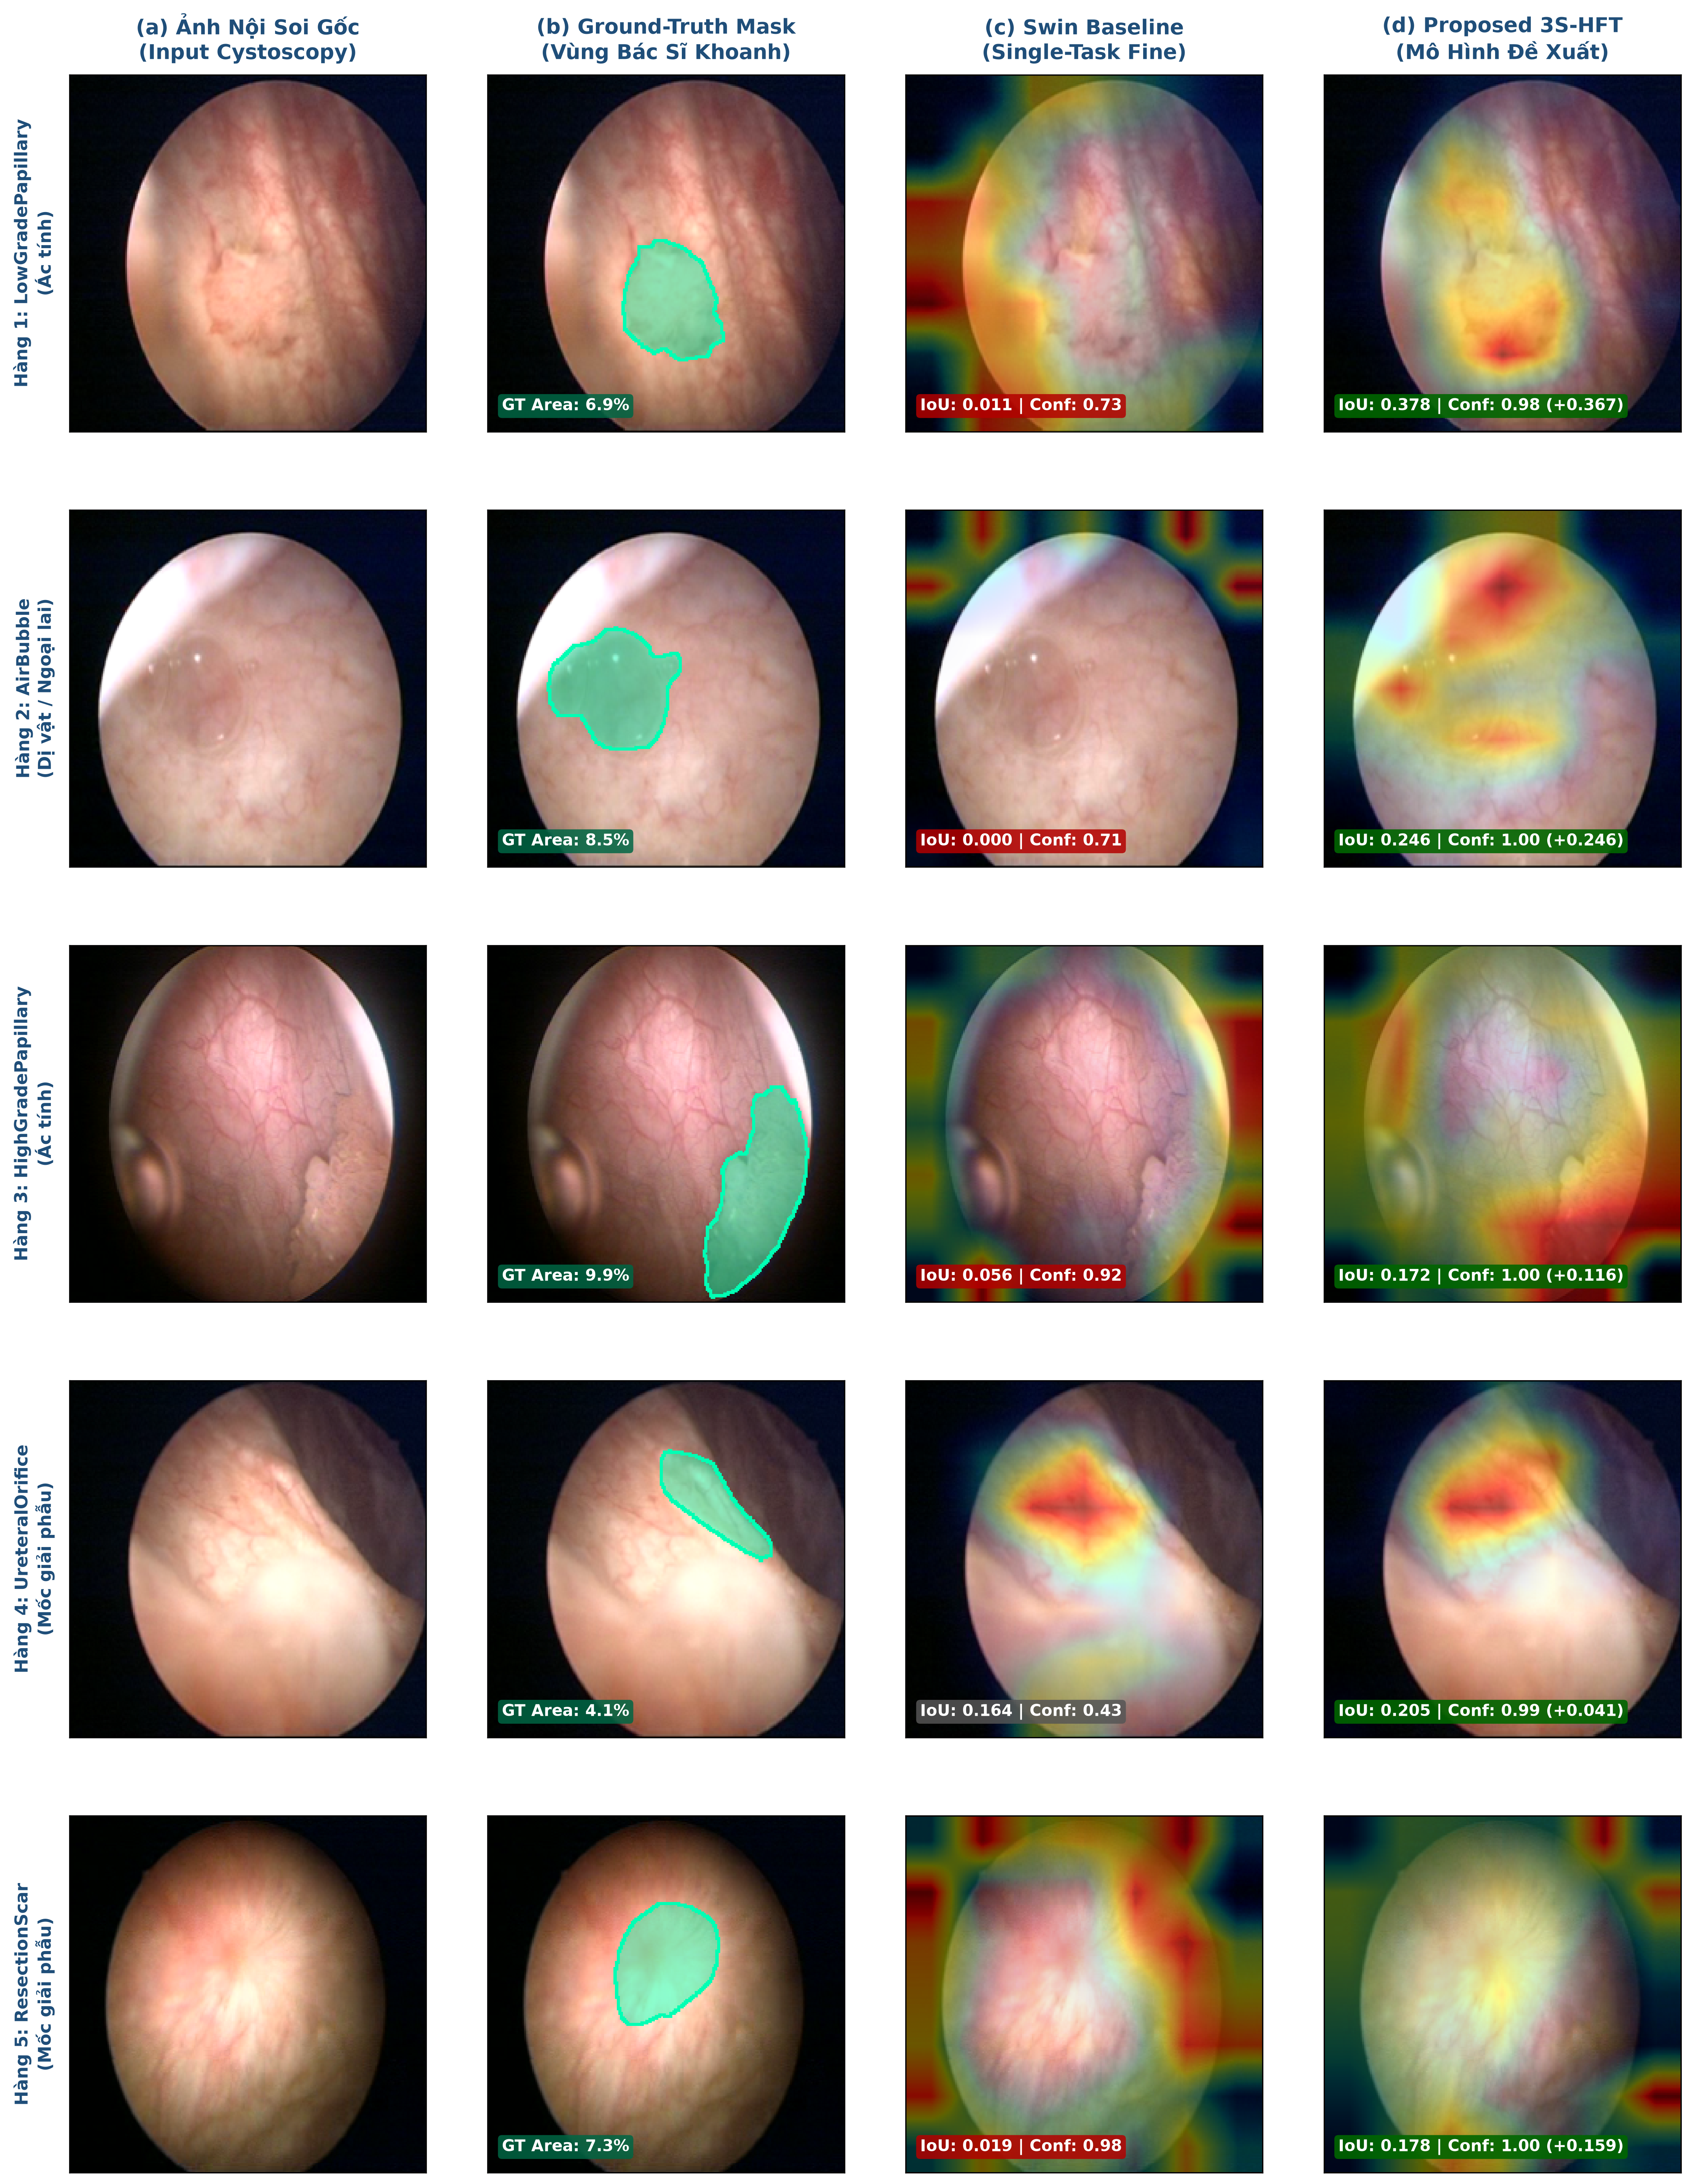
\includegraphics[width=0.88\textwidth]{paper_assets/fig_gradcam_comparison.png}
\caption{Visual explanation comparison using Grad-CAM heatmaps between Single-Task Swin Baseline and \textbf{CystoHier} across 5 fine-grained diagnostic classes with expert Ground-Truth masks: (a) Original WLC endoscopy image; (b) Ground-Truth mask (cyan); (c) Swin Baseline heatmap; (d) \textbf{CystoHier} heatmap showing predicted confidence and Grad-CAM IoU scores.}
\label{fig:gradcam}
\end{figure}

Đánh giá định lượng Grad-CAM IoU với ngưỡng cố định $T=0{,}5$ (Table~\ref{tab:gradcam_iou}) cho thấy mô hình \textbf{CystoHier} đạt IoU trung bình \textbf{23,56\% $\pm$ 7,3\%} so với Swin Baseline (\textbf{5,00\%}), tương ứng mức tăng $+18{,}56$ percentage points (pp). Đặc biệt trên phân lớp tổn thương ác tính \textit{LowGradePapillary}, IoU tăng từ $1{,}12\%$ lên $\mathbf{37{,}78\%}$ ($+36{,}66$ pp). Mô hình đề xuất giảm thiểu kích hoạt giả tại viền đen camera và vùng lóa sáng, cho thấy sự tập trung cao hơn vào các vùng có mức độ tương đồng lớn hơn với Ground-Truth mask.

\begin{table}[H]
\centering
\caption{Quantitative Grad-CAM IoU evaluation on Ground-Truth expert masks. Bold indicates the higher IoU score.}
\label{tab:gradcam_iou}
\begin{adjustbox}{max width=\textwidth}
\begin{tabular}{llccccc}
\toprule
\textbf{Fine-Grained Diagnostic Class} & \textbf{Parent Coarse Group} & \textbf{Evaluation Split} & \textbf{Swin IoU (\%)} & \textbf{CystoHier Conf.} & \textbf{CystoHier IoU (\%)} & \textbf{Gain ($\Delta$ IoU)} \\
\midrule
\textbf{LowGradePapillary} & Malignant & Test Hold-out & 1.12\% & 0.979 & \textbf{37.78\%} & \textbf{+36.66 pp} \\
\textbf{AirBubble} & Foreign bodies & Test Hold-out & 0.00\% & 1.000 & \textbf{24.60\%} & \textbf{+24.60 pp} \\
\textbf{HighGradePapillary} & Malignant & Test Hold-out & 5.56\% & 1.000 & \textbf{17.17\%} & \textbf{+11.61 pp} \\
\textbf{UreteralOrifice} & Landmarks & Test Hold-out & 16.44\% & 0.993 & \textbf{20.50\%} & \textbf{+4.06 pp} \\
\textbf{ResectionScar} & Landmarks & Test Hold-out & 1.87\% & 1.000 & \textbf{17.77\%} & \textbf{+15.90 pp} \\
\midrule
\textbf{Overall Mean} & --- & --- & 5.00\% & 0.994 & \textbf{23.56\%} & \textbf{+18.56 pp (4.71$\times$ rel.)} \\
\bottomrule
\end{tabular}
\end{adjustbox}
\end{table}

\subsection{Benchmark hiệu năng suy luận trên thiết bị phần cứng biên}
Đo lường thời gian thực thi trên phần cứng Apple Silicon MPS FP32 (28,23M tham số, dung lượng bộ nhớ cấp phát 110,8 MiB) được tổng hợp tại Table~\ref{tab:inference_latency}.

\begin{table}[H]
\centering
\caption{Inference latency, throughput, and memory benchmark on edge hardware (MPS FP32).}
\label{tab:inference_latency}
\begin{adjustbox}{max width=\textwidth}
\begin{tabular}{lcccc}
\toprule
\textbf{Batch Size Configuration} & \textbf{Forward Model (ms/img)} & \textbf{Forward Throughput (FPS)} & \textbf{End-to-End Pipeline (ms)} & \textbf{Allocated Memory} \\
\midrule
\textbf{Batch = 1 (Real-time Single Image)} & \textbf{12.08 $\pm$ 0.95 ms} & \textbf{82.78 FPS} & \textbf{15.00 $\pm$ 1.12 ms (66.67 FPS)} & 110.83 MiB \\
Batch = 8 (Mini-batch) & 10.17 $\pm$ 0.42 ms & 98.36 FPS & --- & 113.99 MiB \\
Batch = 32 (High Throughput) & 9.95 $\pm$ 0.38 ms & 100.46 FPS & --- & 128.00 MiB \\
\bottomrule
\end{tabular}
\end{adjustbox}
\end{table}

Thông lượng suy luận toàn trình đo được là \textbf{66,67 FPS} (độ trễ 15,00 ms/ảnh), cho thấy mô hình hoàn toàn đáp ứng dư dả tài nguyên tính toán cho việc xử lý khung hình thời gian thực trong phẫu thuật nội soi.

\section{Thảo luận và Hạn chế}
\label{sec:discussion}

Nghiên cứu xác lập sự tương hỗ mật thiết giữa các trụ cột kỹ thuật của \textbf{CystoHier}: (1) \textit{Swin-Tiny} cung cấp không gian đặc trưng biểu mô đa phân giải; (2) \textit{Smoothed Balanced Softmax} cân bằng phân phối theo số lượng bệnh nhân; (3) \textit{Curriculum Hierarchy Warmup} giải phóng ràng buộc phả hệ sớm; (4) \textit{Supervised Contrastive Regularization} co cụm cấu trúc chi tiết; và (5) \textit{Hierarchical Marginalization} tận dụng xác suất từ phân lớp chi tiết để hiệu chỉnh nhóm cha. 

Phân tích ma trận nhầm lẫn lâm sàng chỉ ra rằng các trường hợp chẩn đoán sai lệch giữa nhóm \textit{Non-malignant} và \textit{Malignant} (26/32 ảnh) chủ yếu do mô hình có xu hướng cảnh báo an toàn (\textit{overcalling}) nhằm tránh bỏ sót các tổn thương tiền ung thư. Xu hướng dự đoán thận trọng này có thể hữu ích trong tầm soát nhằm giảm thiểu nguy cơ bỏ sót tổn thương; tuy nhiên, giá trị lâm sàng thực tế và tác động của dương tính giả cần được đánh giá trong các nghiên cứu tiền cứu.

\noindent \textbf{Hạn chế và hướng phát triển:} Mặc dù đã kiểm định thành công trên tập Lazo et al., nghiên cứu hiện tại vẫn mang tính chất hồi cứu trên cỡ mẫu ngoại kiểm 23 bệnh nhân. Các nghiên cứu tiếp theo cần mở rộng sang thử nghiệm tiền cứu đa trung tâm và khảo sát các kiến trúc Temporal Video Transformer cho chuỗi video liên tục.

\section{Kết luận}
\label{sec:conclusion}
Bài báo đã đề xuất khung phương pháp \textbf{CystoHier} kết hợp tinh chỉnh tách rời ba giai đoạn, \textbf{Curriculum Hierarchy Warmup} và \textbf{Hierarchical Marginalization} cho bài toán phân loại phân cấp nội soi bàng quang trên dữ liệu mất cân bằng dài đuôi CystoDS. Mô hình cải thiện nhất quán phân loại chi tiết (Fine Macro-F1 0,6450 $\pm$ 0,1105) và tính nhất quán phả hệ (89,52\% $\pm$ 3,80\%) trên tập kiểm định độc lập bệnh nhân, đồng thời duy trì khả năng phân loại nhị phân vững chắc (Binary AUROC 0,9986 $\pm$ 0,0002). Đánh giá zero-shot trên tập ngoại kiểm độc lập Lazo et al. khẳng định năng lực tổng quát hóa cross-dataset tốt, đặc biệt trên ảnh NBI và tổn thương NTL. Mô hình đạt thông lượng 66,7 FPS end-to-end trên phần cứng biên và cải thiện độ trùng khớp Grad-CAM IoU giải phẫu. Các kết quả này chứng minh tính khả thi của việc học phân cấp dài đuôi trong chẩn đoán hình ảnh nội soi bàng quang, trong khi các thử nghiệm tiền cứu đa trung tâm vẫn là bước cần thiết tiếp theo trước khi triển khai lâm sàng thực tế.

\subsubsection*{Lời cảm ơn.}
Nghiên cứu này được thực hiện tại Trường Đại học FPT, Phân hiệu Đà Nẵng. Các tác giả chân thành cảm ơn sự hỗ trợ học thuật và môi trường nghiên cứu từ nhà trường.

\subsubsection*{Tuyên bố xung đột lợi ích.}
Các tác giả tuyên bố không có xung đột lợi ích liên quan đến nội dung của bài báo này.

%
% ---- Bibliography ----
%
\begin{thebibliography}{16}

\bibitem{ref_lee2026cystods}
Lee, T.J., Qiu, L., Long, J., Mach, K.E., Peterson, D., Yao, Q., Shkolyar, E., Islam, M.T., Xing, L., Liao, J.C.: CystoDS: a multiclass endoscopy image dataset for artificial intelligence-assisted bladder cancer detection. Scientific Data \textbf{13}(1), 1--14 (2026). \doi{10.1038/s41597-026-06887-z}

\bibitem{ref_shkolyar2019augmented}
Shkolyar, E., Jia, X., Chang, T.C., Trivedi, D.V., Mach, K.E., Meng, M.Q.H., Xing, L., Liao, J.C.: Augmented Bladder Tumor Detection Using Deep Learning. European Urology \textbf{76}(6), 714--718 (2019). \doi{10.1016/j.eururo.2019.08.032}

\bibitem{ref_wu2022multicenter}
Wu, S., Chen, X., Pan, J., Zhou, Z., Shen, C., Wang, Z., Huang, J.: An Artificial Intelligence System for the Detection of Bladder Cancer via Cystoscopy: A Multicenter Diagnostic Study. Journal of the National Cancer Institute \textbf{114}(2), 220--227 (2022). \doi{10.1093/jnci/djab179}

\bibitem{ref_lazo2023semisupervised}
Lazo Sanchez, J., Rosa, B., Cattellani, M., Ferro, M., De Cobelli, O., Mateus, D.: Semi-supervised Bladder Tissue Classification in Multi-Domain Endoscopic Images. IEEE Transactions on Biomedical Engineering \textbf{70}(10), 2822--2833 (2023). \doi{10.1109/TBME.2023.3265679}

\bibitem{ref_jia2023transformer}
Jia, X., Shkolyar, E., Laurie, M.A., Mach, K.E., Meng, M.QH., Liao, J.C., Xing, L.: Tumor detection under cystoscopy with transformer-augmented deep learning algorithm. Physics in Medicine \& Biology \textbf{68}(16), 165013 (2023). \doi{10.1088/1361-6560/ace499}

\bibitem{ref_abdelaziz2025efficientnet}
Abd El-Aziz, A.A., Mahmood, M.A., Abd El-Ghany, S.: EfficientNet-B3-Based Automated Deep Learning Framework for Multiclass Endoscopic Bladder Tissue Classification. Diagnostics \textbf{15}(19), 2515 (2025). \doi{10.3390/diagnostics15192515}

\bibitem{ref_wang2026narrowband}
Wang, Y., Liang, H., Zhang, Y., et al.: Artificial intelligence diagnostics for bladder tumor identification and grade prediction depend on narrow band imaging cystoscopy. iScience \textbf{29}(2), 114309 (2026). \doi{10.1016/j.isci.2025.114309}

\bibitem{ref_zhang2026multiarch}
Zhang, F., An, J., Zhao, L., et al.: Artificial Intelligence-Powered Cystoscopy Diagnostic Support System: Clinical Application of Multiarchitecture Deep Learning Models. Journal of Endourology \textbf{40}(8), 925--934 (2026). \doi{10.1177/08927790261450807}

\bibitem{ref_liu2021swin}
Liu, Z., Lin, Y., Cao, Y., Hu, H., Wei, Y., Zhang, Z., Lin, S., Guo, B.: Swin Transformer: Hierarchical Vision Transformer using Shifted Windows. In: Proceedings of the IEEE/CVF International Conference on Computer Vision (ICCV), pp. 10012--10022 (2021). \doi{10.1109/ICCV48922.2021.00986}

\bibitem{ref_ren2020balanced}
Ren, J., Yu, C., Ma, X., Zhao, H., Yi, S.: Balanced Meta-Softmax for Long-Tailed Visual Recognition. In: Advances in Neural Information Processing Systems (NeurIPS), vol. 33, pp. 4175--4186 (2020)

\bibitem{ref_khosla2020supervised}
Khosla, P., Teterwak, P., Wang, C., Sarna, A., Tian, Y., Isola, P., Maschinot, A., Liu, C., Krishnan, D.: Supervised Contrastive Learning. In: Advances in Neural Information Processing Systems (NeurIPS), vol. 33, pp. 18661--18673 (2020)

\bibitem{ref_kang2020decoupling}
Kang, B., Xie, S., Rohrbach, M., Yan, Z., Gordo, A., Feng, J., Kalantidis, Y.: Decoupling Representation and Classifier for Long-Tailed Recognition. In: International Conference on Learning Representations (ICLR) (2020)

\bibitem{ref_menon2021logit}
Menon, A.K., Jayasumana, S., Rawat, A.S., Jain, H., Veit, A., Kumar, S.: Long-tail learning via logit adjustment. In: International Conference on Learning Representations (ICLR) (2021)

\bibitem{ref_he2016resnet}
He, K., Zhang, X., Ren, S., Sun, J.: Deep Residual Learning for Image Recognition. In: Proceedings of the IEEE Conference on Computer Vision and Pattern Recognition (CVPR), pp. 770--778 (2016). \doi{10.1109/CVPR.2016.90}

\bibitem{ref_xie2017resnext}
Xie, S., Girshick, R., Dollár, P., Tu, Z., He, K.: Aggregated Residual Transformations for Deep Neural Networks. In: Proceedings of the IEEE Conference on Computer Vision and Pattern Recognition (CVPR), pp. 1492--1500 (2017). \doi{10.1109/CVPR.2017.634}

\bibitem{ref_sun2019hrnet}
Sun, K., Xiao, B., Liu, D., Wang, J.: Deep High-Resolution Representation Learning for Human Pose Estimation. In: Proceedings of the IEEE/CVF Conference on Computer Vision and Pattern Recognition (CVPR), pp. 5693--5703 (2019). \doi{10.1109/CVPR.2019.00584}

\end{thebibliography}
\end{document}
